% Saberes básicos (LOMLOE) asociados a esta unidad
%
% Bloque B. La materia
%   - Teoría cinético-molecular: aplicación a observaciones sobre la materia
%     explicando la formación de mezclas y disoluciones — la unidad clasifica
%     mezclas homogéneas/heterogéneas, disoluciones, coloides y emulsiones a
%     partir del tamaño de partícula.
%   - Experimentos relacionados con los sistemas materiales: conocimiento y
%     descripción de sus propiedades, su composición y su clasificación —
%     se distinguen sustancias puras de mezclas y se caracteriza cada tipo
%     mediante propiedades como el punto de fusión o la concentración.
%   - Estructura atómica: desarrollo histórico de los modelos atómicos,
%     existencia, formación y propiedades de los isótopos y ordenación de los
%     elementos en la tabla periódica — se tratan los modelos de Dalton,
%     Thomson, Rutherford y Bohr, el número atómico, el número másico, los
%     isótopos y la organización en periodos y grupos.
%   - Principales compuestos químicos: su formación y sus propiedades físicas
%     y químicas, valoración de sus aplicaciones. Masa atómica y masa
%     molecular — se introduce el concepto de masa atómica al presentar
%     protones, neutrones e isótopos.
%
% Bloque A. Las destrezas científicas básicas
%   - El lenguaje científico: unidades del Sistema Internacional — se usan de
%     forma consistente las unidades de masa y volumen (g, mL, g/L) al
%     calcular la concentración de las disoluciones.
%
% Esta unidad no desarrolla contenidos propios de los bloques C (la energía)
% ni D (la interacción), centrados en calor, electricidad, cinemática y
% fuerzas. Tampoco aborda el bloque E (el cambio), reservado a las
% reacciones químicas y su conservación de la masa, que se trabaja en otra
% unidad del curso.
%
% (Traducción al español de Unit_3_Diversity_of_Matter.tex. La sección comentada
%  «How chemical compounds are named» del original no se traduce: la formulación está en la Unidad 4.)

\spacing{1.3}
\raggedbottom % pages with large figures end where the text ends (no stretched gaps between boxes)

\section{Sustancias puras y mezclas}

Mira a tu alrededor: el agua, el aire, un lápiz, un bocadillo\ldots{} Algunas de estas cosas están formadas por \textbf{una} sola sustancia y otras están formadas por \textbf{varias} sustancias mezcladas.

\begin{figure}[H]
    \centering
    % [FIGURA ORIGINAL] \includegraphics[width=\textwidth]{Unit_3/matter_classification}
    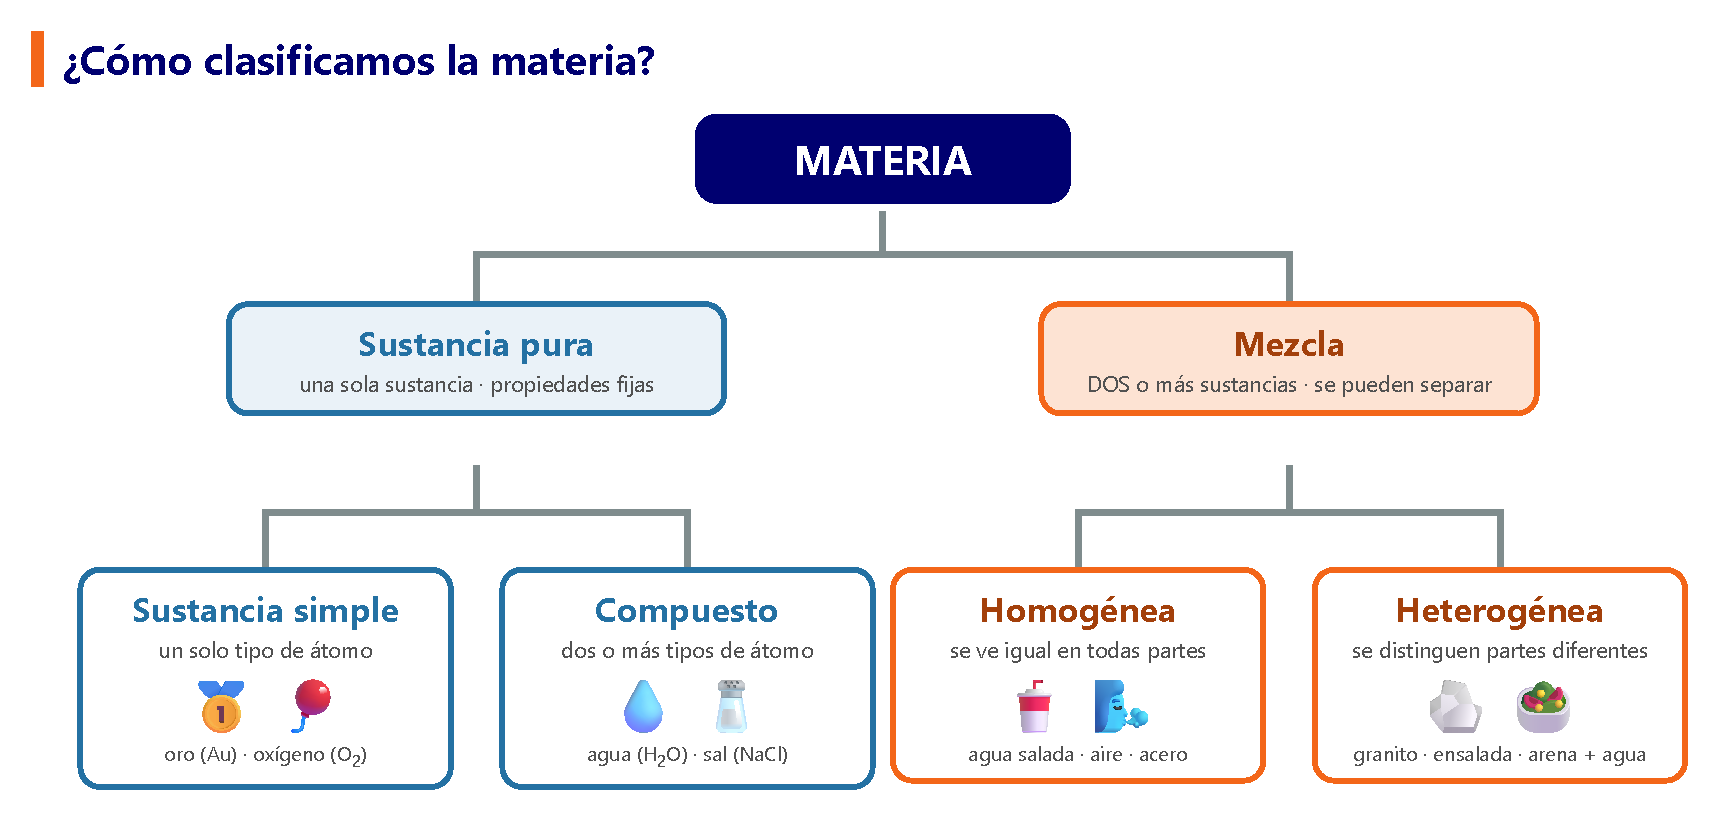
\includegraphics[width=\textwidth]{FigurasSVG/Unit_3_Diversity_of_Matter/pdf/matter_classification_es.pdf}
    \caption{Clasificación de la materia.}
    \label{fig:u3_matter_classification}
\end{figure}

\begin{definition}[Sustancia pura]
    Es la materia formada por \textbf{una sola} sustancia. Tiene unas propiedades fijas y características (por ejemplo, una temperatura de fusión fija). Puede ser una \textbf{sustancia simple} (un solo tipo de átomo) o un \textbf{compuesto} (dos o más tipos de átomos).
\end{definition}

\begin{definition}[Mezcla]
    Es la materia formada por \textbf{dos o más} sustancias. Es \textbf{homogénea} si tiene el mismo aspecto en todas sus partes (incluso al microscopio), y \textbf{heterogénea} si podemos distinguir partes diferentes.
\end{definition}

\begin{impt}
    \textbf{¿Sustancia pura o mezcla?} Mide su temperatura de fusión. El hielo puro siempre funde a \qty{0}{\celsius}; distintas muestras de mantequilla (una mezcla) funden a temperaturas algo diferentes, porque su composición no es fija.
\end{impt}

\begin{exercise}
    Clasifica cada ejemplo de materia según su \textbf{aspecto} (homogéneo o heterogéneo) y su \textbf{composición} (sustancia pura o mezcla): azúcar, agua salada, granito, oxígeno gaseoso, leche.
    \begin{solu}
        \begin{center}
            \begin{tabular}{lll}
                \toprule
                \textbf{Materia} & \textbf{Aspecto} & \textbf{Composición} \\
                \midrule
                Azúcar & Homogéneo & Sustancia pura \\
                Agua salada & Homogéneo & Mezcla \\
                Granito & Heterogéneo & Mezcla \\
                Oxígeno gaseoso & Homogéneo & Sustancia pura \\
                Leche & Parece homogénea, pero es un coloide (heterogénea) & Mezcla \\
                \bottomrule
            \end{tabular}
        \end{center}
    \end{solu}
\end{exercise}

\begin{exercise}
    Indica si cada ejemplo tiene un aspecto homogéneo o heterogéneo: aire, agua hirviendo, humo, yogur, azúcar, granizado de limón, leche con cacao, papel escrito.
    \begin{solu}
        \textbf{Homogéneos}: aire, azúcar. \\
        \textbf{Heterogéneos}: agua hirviendo (burbujas de gas en el líquido), humo (partículas sólidas en el aire), yogur, granizado de limón, leche con cacao, papel escrito.
    \end{solu}
\end{exercise}

\begin{exercise}
    Decide si cada sistema es una \textbf{sustancia pura} o una \textbf{mezcla} y justifica brevemente tu respuesta: a) agua mineral; b) oxígeno gaseoso (\ch{O2}); c) zumo de naranja con pulpa; d) azufre en polvo (\ch{S}).
    \begin{solu}
        \begin{enumerate}[label=\alph*)]
            \item \textbf{Mezcla}: agua con varios minerales disueltos.
            \item \textbf{Sustancia pura} (sustancia simple): solo átomos de oxígeno.
            \item \textbf{Mezcla} (heterogénea): zumo, agua y pulpa que se ve.
            \item \textbf{Sustancia pura} (sustancia simple): solo átomos de azufre.
        \end{enumerate}
    \end{solu}
\end{exercise}

%----------------------------------------------------------------------------------------

\section{Mezclas homogéneas y heterogéneas}

Las mezclas se clasifican según \textbf{lo que vemos}: ¿podemos distinguir sus componentes solo con mirarlas, o no?

\subsection{Mezclas homogéneas}

\begin{definition}[Mezcla homogénea]
    Es una mezcla cuyos componentes \textbf{no se pueden distinguir a simple vista}: tiene el mismo aspecto (uniforme) en todas sus partes, y cualquier muestra que tomemos tiene la misma composición y las mismas propiedades.
\end{definition}

\begin{example}
    Algunas mezclas homogéneas que usamos a diario:
    \begin{itemize}
        \item El \textbf{agua salada} o el \textbf{azúcar disuelto en el té}: cuando la sal o el azúcar se han disuelto, ya no los vemos.
        \item El \textbf{aire}: es una mezcla de nitrógeno, oxígeno, argón, dióxido de carbono y otros gases, pero no vemos ninguno de ellos.
        \item El \textbf{agua mineral} y el \textbf{vinagre}: parecen un único líquido transparente.
        \item El \textbf{acero} y el \textbf{bronce}: metales tan bien mezclados que parecen un único metal.
    \end{itemize}
\end{example}

Las mezclas homogéneas más importantes son las \textbf{disoluciones}, que estudiamos con detalle a continuación.

\subsubsection{Disoluciones}

\begin{definition}[Disolución]
    Es una mezcla \textbf{homogénea} de dos o más sustancias. El \textbf{disolvente} es el componente que está en mayor cantidad; el \textbf{soluto} (o los solutos) está en menor cantidad.
\end{definition}

\begin{figure}[H]
    \centering
    % [FIGURA ORIGINAL] \includegraphics[width=\textwidth]{Unit_3/solution_parts}
    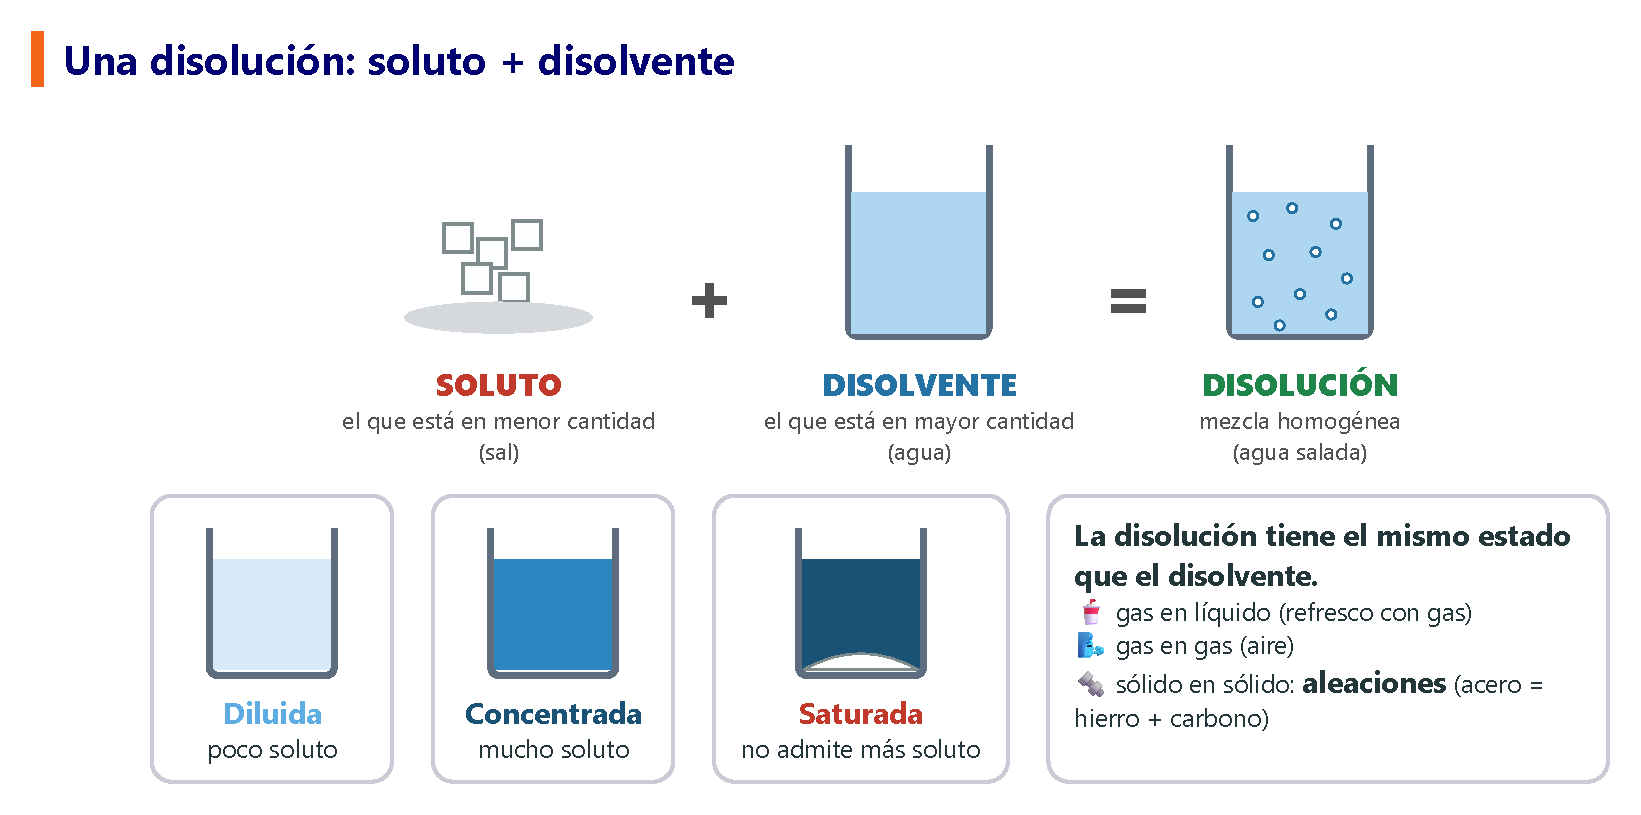
\includegraphics[width=\textwidth]{FigurasSVG/Unit_3_Diversity_of_Matter/pdf/solution_parts_es.pdf}
    \caption{Las partes de una disolución, y disoluciones diluidas, concentradas y saturadas.}
    \label{fig:u3_solution_parts}
\end{figure}

\begin{impt}
    Una disolución tiene siempre \textbf{un} disolvente, pero puede tener \textbf{más de un soluto}. Por ejemplo:
    \begin{itemize}
        \item El \textbf{agua de mar}: el disolvente es el agua, y los solutos son muchas sales distintas (cloruro de sodio, cloruro de magnesio, sulfato de calcio\ldots).
        \item Un \textbf{refresco}: el disolvente es el agua, y los solutos son el azúcar, el dióxido de carbono (las burbujas), los colorantes y los aromas.
        \item El \textbf{aire}: el disolvente es el nitrógeno, y los solutos son el oxígeno, el argón, el dióxido de carbono y el vapor de agua.
    \end{itemize}
\end{impt}

\begin{definition}[Aleación]
    Es una disolución sólida de dos o más metales (o de un metal y otro elemento) que se fabrica para mejorar las propiedades del metal puro. Ejemplos: el acero (hierro + carbono) y el bronce (cobre + estaño).
\end{definition}

\begin{exercise}
    Indica para cada mezcla el estado físico del soluto y del disolvente: aire, azúcar en agua, acero, agua con gas, infusión de manzanilla.
    \begin{solu}
        \begin{center}
            \begin{tabular}{lll}
                \toprule
                \textbf{Mezcla} & \textbf{Soluto} & \textbf{Disolvente} \\
                \midrule
                Aire & Gas (oxígeno, etc.) & Gas (nitrógeno) \\
                Azúcar en agua & Sólido & Líquido \\
                Acero & Sólido (carbono) & Sólido (hierro) \\
                Agua con gas & Gas (\ch{CO2}) & Líquido \\
                Infusión de manzanilla & Sólido/líquido & Líquido \\
                \bottomrule
            \end{tabular}
        \end{center}
    \end{solu}
\end{exercise}

\begin{exercise}
    Se prepara una disolución mezclando \qty{5}{\mL} de etanol con \qty{45}{\mL} de agua. Identifica el soluto y el disolvente. ¿Esta disolución está más o menos concentrada que otra preparada con \qty{20}{\mL} de etanol y \qty{30}{\mL} de agua?
    \begin{solu}
        El etanol está en menor cantidad, así que es el \textbf{soluto}; el agua es el \textbf{disolvente}. \\
        La primera disolución tiene \qty{5}{\mL} de etanol en \qty{50}{\mL}, y la segunda \qty{20}{\mL} en \qty{50}{\mL}, así que la primera está \textbf{más diluida} (menos concentrada).
    \end{solu}
\end{exercise}

\begin{exercise}
    Pon dos ejemplos de disoluciones que haya en casa para cada caso: a) sólido disuelto en líquido; b) líquido disuelto en líquido; c) gas disuelto en líquido.
    \begin{solu}
        \begin{enumerate}[label=\alph*)]
            \item Azúcar en el café; sal en la sopa.
            \item Vinagre (ácido acético en agua); anticongelante en agua.
            \item Agua con gas (\ch{CO2} en agua); oxígeno disuelto en el agua de un acuario.
        \end{enumerate}
    \end{solu}
\end{exercise}

\subsubsection{Concentración de una disolución}

\begin{definition}[Concentración]
    Es la cantidad de soluto disuelta en una cantidad determinada de disolución.
\end{definition}

Antes de calcular cualquier concentración, debemos tener muy claro qué es la \textbf{disolución}. La disolución es \textbf{todo}: el soluto (o los solutos) \textbf{más} el disolvente.

\begin{figure}[H]
    \centering
    % [FIGURA ORIGINAL] \includegraphics[width=\textwidth]{Unit_3/solution_sum}
    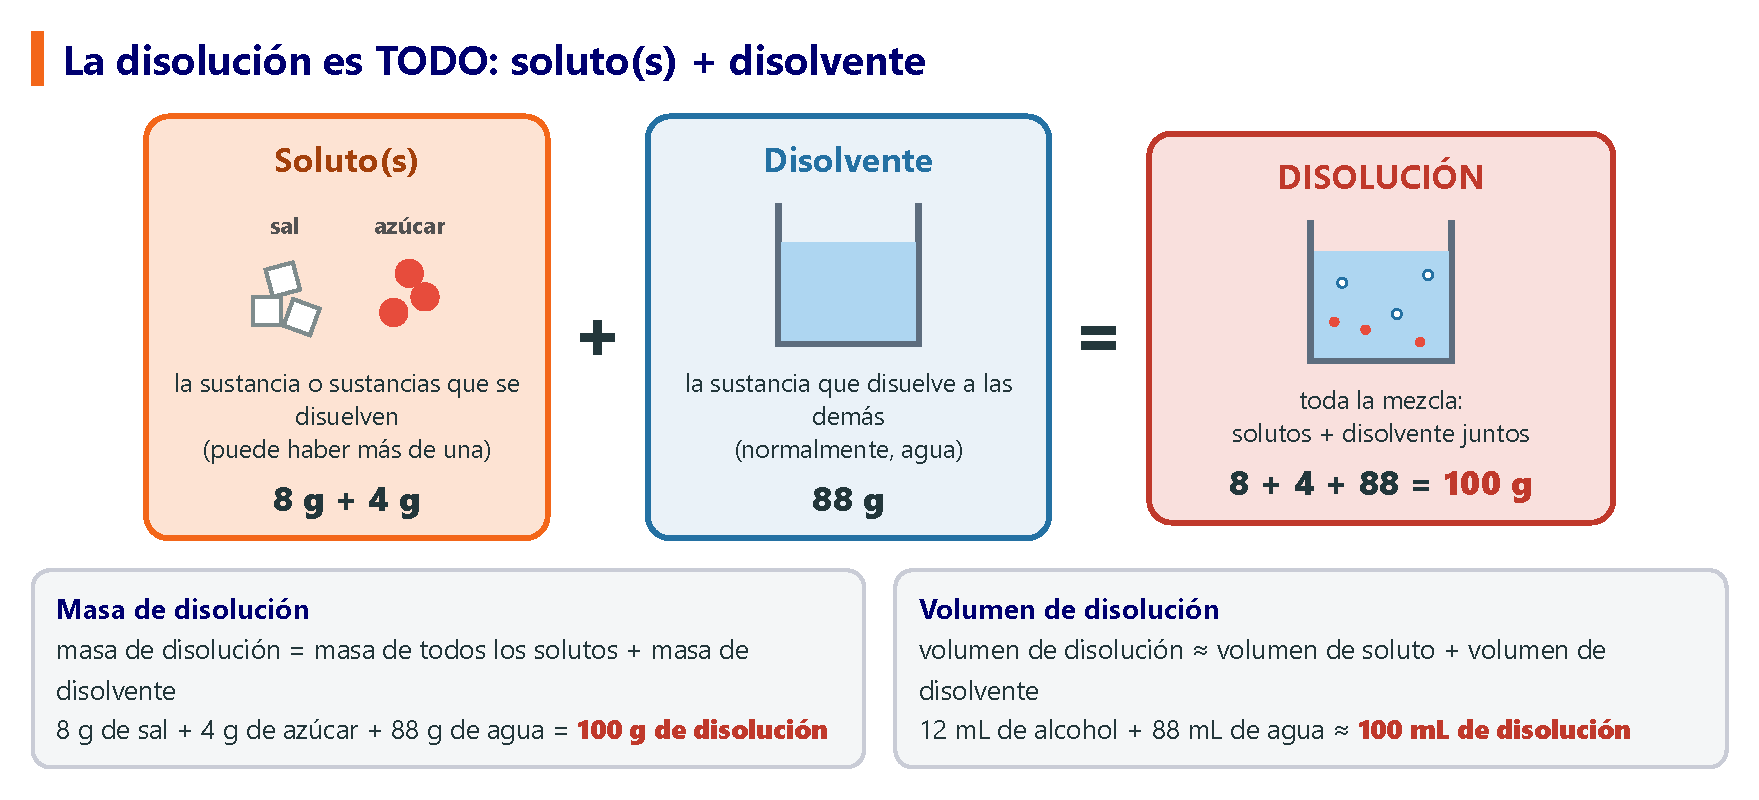
\includegraphics[width=\textwidth]{FigurasSVG/Unit_3_Diversity_of_Matter/pdf/solution_sum_es.pdf}
    \caption{La disolución es la suma de todos los solutos y el disolvente.}
    \label{fig:u3_solution_sum}
\end{figure}

\begin{impt}
    \negsubro{Disolución = soluto(s) + disolvente}
    \begin{equation*}
        \text{masa de disolución} = \text{masa de soluto(s)} + \text{masa de disolvente}
    \end{equation*}
    \begin{equation*}
        \text{volumen de disolución} \approx \text{volumen de soluto} + \text{volumen de disolvente}
    \end{equation*}
    En todas las fórmulas de la concentración, \textbf{debajo} de la raya de fracción va la \textbf{disolución}, \textbf{nunca} el disolvente solo. Si el ejercicio te da el soluto y el disolvente por separado, primero \textbf{súmalos} para obtener la disolución.
\end{impt}

Usaremos tres formas de expresar la concentración de una disolución:

\begin{figure}[H]
    \centering
    % [FIGURA ORIGINAL] \includegraphics[width=\textwidth]{Unit_3/concentration}
    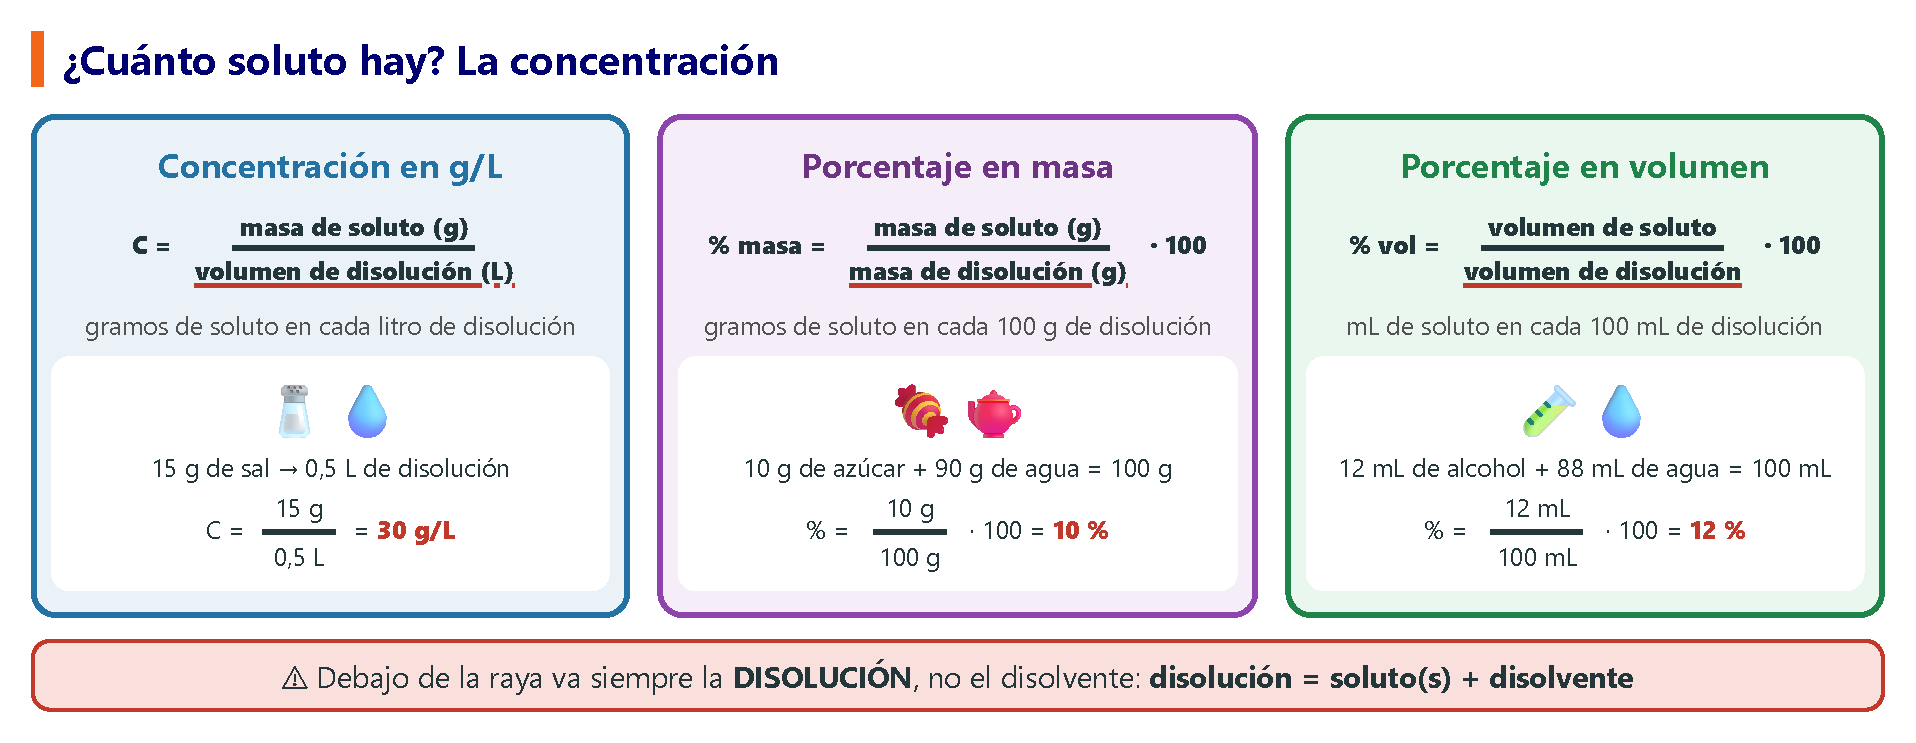
\includegraphics[width=\textwidth]{FigurasSVG/Unit_3_Diversity_of_Matter/pdf/concentration_es.pdf}
    \caption{Tres formas de expresar la concentración.}
    \label{fig:u3_concentration}
\end{figure}

\begin{equation*}
    C\,(\unit{\g\per\litre}) = \dfrac{\text{masa de soluto (g)}}{\text{volumen de disolución (L)}}
\end{equation*}
\begin{equation*}
    \%\text{ en masa} = \dfrac{\text{masa de soluto (g)}}{\text{masa de disolución (g)}} \cdot 100
    \qquad\qquad
    \%\text{ en volumen} = \dfrac{\text{volumen de soluto (mL)}}{\text{volumen de disolución (mL)}} \cdot 100
\end{equation*}

\begin{impt}
    \begin{itemize}
        \item La \textbf{concentración en g/L} nos dice cuántos \textbf{gramos} de soluto hay en cada \textbf{litro} de disolución. El volumen tiene que estar en \textbf{litros}.
        \item El \textbf{porcentaje en masa} nos dice cuántos \textbf{gramos} de soluto hay en cada \textbf{\qty{100}{\g}} de disolución. Las dos masas tienen que estar en la \textbf{misma unidad}.
        \item El \textbf{porcentaje en volumen} nos dice cuántos \textbf{mililitros} de soluto hay en cada \textbf{\qty{100}{\mL}} de disolución. Se usa cuando el soluto es un \textbf{líquido} (por ejemplo, el alcohol del vino). Los dos volúmenes tienen que estar en la \textbf{misma unidad}.
    \end{itemize}
\end{impt}

\begin{example}
    \textbf{Concentración en g/L. Se disuelven \qty{15}{\g} de sal en agua hasta obtener \qty{500}{\mL} de disolución. ¿Cuál es la concentración en g/L?}
    \begin{enumerate}[label=\numberballmDarkTeal]
        \item Datos: masa de soluto \(= \qty{15}{\g}\); volumen de disolución \(= \qty{500}{\mL}\). Incógnita: \(C\).
        \item El volumen tiene que estar en litros: \(\num{500}\,\unit{\mL} \cdot \dfrac{\qty{1}{\litre}}{\qty{e3}{\mL}} = \qty{0.5}{\litre}\).
        \item Fórmula: \(C = \dfrac{\text{masa de soluto}}{\text{volumen de disolución}}\).
        \item \(C = \dfrac{\qty{15}{\g}}{\qty{0.5}{\litre}} = \textcolor{red}{\qty{30}{\g\per\litre}}\). Hay \qty{30}{\g} de sal en cada litro de disolución.
    \end{enumerate}
\end{example}

\begin{example}
    \textbf{Porcentaje en masa. Se disuelven \qty{20}{\g} de azúcar en \qty{180}{\g} de agua. ¿Cuál es el porcentaje en masa de azúcar?}
    \begin{enumerate}[label=\numberballmDarkTeal]
        \item Datos: masa de soluto (azúcar) \(= \qty{20}{\g}\); masa de \textbf{disolvente} (agua) \(= \qty{180}{\g}\). Incógnita: \% en masa.
        \item \textbf{Cuidado}: \qty{180}{\g} es el disolvente, \textbf{no} la disolución. Los sumamos: \\
        masa de disolución \(= \qty{20}{\g} + \qty{180}{\g} = \qty{200}{\g}\).
        \item Fórmula: \(\%\text{ en masa} = \dfrac{\text{masa de soluto}}{\text{masa de disolución}} \cdot 100\).
        \item \(\%\text{ en masa} = \dfrac{\qty{20}{\g}}{\qty{200}{\g}} \cdot 100 = \textcolor{red}{\qty{10}{\percent}}\). Hay \qty{10}{\g} de azúcar en cada \qty{100}{\g} de disolución.
    \end{enumerate}
\end{example}

\begin{example}
    \textbf{Porcentaje en volumen. Se prepara una disolución mezclando \qty{30}{\mL} de alcohol con \qty{120}{\mL} de agua. ¿Cuál es el porcentaje en volumen de alcohol?}
    \begin{enumerate}[label=\numberballmDarkTeal]
        \item Datos: volumen de soluto (alcohol) \(= \qty{30}{\mL}\); volumen de \textbf{disolvente} (agua) \(= \qty{120}{\mL}\). Incógnita: \% en volumen.
        \item Volumen de disolución \(= \qty{30}{\mL} + \qty{120}{\mL} = \qty{150}{\mL}\).
        \item Fórmula: \(\%\text{ en volumen} = \dfrac{\text{volumen de soluto}}{\text{volumen de disolución}} \cdot 100\).
        \item \(\%\text{ en volumen} = \dfrac{\qty{30}{\mL}}{\qty{150}{\mL}} \cdot 100 = \textcolor{red}{\qty{20}{\percent}}\). Hay \qty{20}{\mL} de alcohol en cada \qty{100}{\mL} de disolución.
    \end{enumerate}
\end{example}

\begin{didyouknow}
    Las etiquetas de las bebidas indican el porcentaje en volumen de alcohol: «13\,\% vol.» en una botella de vino significa que cada \qty{100}{\mL} de vino contienen \qty{13}{\mL} de alcohol.
\end{didyouknow}

\begin{exercise}
    \textbf{Concentración en g/L.} Calcula:
    \begin{enumerate}[label=\letraminuscula]
        \item La concentración en g/L de una disolución preparada disolviendo \qty{20}{\g} de azúcar en agua hasta un volumen de \qty{400}{\mL}.
        \item La concentración en g/L de una disolución que contiene \qty{6}{\g} de sal en \qty{1.5}{\litre} de disolución.
        \item La masa de sal que hay en una botella de \qty{500}{\mL} de suero fisiológico cuya concentración es \qty{9}{\g\per\litre}.
    \end{enumerate}
    \begin{solu}
        \begin{enumerate}[label=\alph*)]
            \item \(V = \qty{400}{\mL} = \qty{0.4}{\litre}\); \(C = \dfrac{\qty{20}{\g}}{\qty{0.4}{\litre}} = \qty{50}{\g\per\litre}\).
            \item \(C = \dfrac{\qty{6}{\g}}{\qty{1.5}{\litre}} = \qty{4}{\g\per\litre}\).
            \item \(V = \qty{0.5}{\litre}\); masa de soluto \(= C \cdot V = \qty{9}{\g\per\litre} \cdot \qty{0.5}{\litre} = \qty{4.5}{\g}\).
        \end{enumerate}
    \end{solu}
\end{exercise}

\begin{exercise}
    \textbf{Porcentaje en masa.} Calcula:
    \begin{enumerate}[label=\letraminuscula]
        \item El porcentaje en masa de una disolución preparada con \qty{15}{\g} de sal y \qty{135}{\g} de agua.
        \item El porcentaje en masa de cada soluto en una disolución preparada con \qty{2}{\g} de sal, \qty{3}{\g} de azúcar y \qty{95}{\g} de agua.
        \item La masa de soluto y la masa de agua que hay en \qty{300}{\g} de una disolución al \qty{5}{\percent} en masa.
    \end{enumerate}
    \begin{solu}
        \begin{enumerate}[label=\alph*)]
            \item Masa de disolución \(= 15 + 135 = \qty{150}{\g}\); \(\%\text{ en masa} = \dfrac{\qty{15}{\g}}{\qty{150}{\g}} \cdot 100 = \qty{10}{\percent}\).
            \item Masa de disolución \(= 2 + 3 + 95 = \qty{100}{\g}\) (todos los solutos y el disolvente). Sal: \(\dfrac{\qty{2}{\g}}{\qty{100}{\g}} \cdot 100 = \qty{2}{\percent}\); azúcar: \(\dfrac{\qty{3}{\g}}{\qty{100}{\g}} \cdot 100 = \qty{3}{\percent}\).
            \item Masa de soluto \(= \qty{300}{\g} \cdot \dfrac{5}{100} = \qty{15}{\g}\); masa de agua \(= 300 - 15 = \qty{285}{\g}\).
        \end{enumerate}
    \end{solu}
\end{exercise}

\begin{exercise}
    \textbf{Porcentaje en volumen.} Calcula:
    \begin{enumerate}[label=\letraminuscula]
        \item El porcentaje en volumen de una disolución preparada mezclando \qty{30}{\mL} de alcohol con \qty{220}{\mL} de agua.
        \item El volumen de alcohol que hay en una botella de vino de \qty{750}{\mL} con la etiqueta «\qty{13}{\percent} vol.».
        \item Un gel hidroalcohólico tiene un \qty{70}{\percent} en volumen de alcohol. ¿Cuántos mililitros de alcohol y de agua hay en un bote de \qty{200}{\mL}?
    \end{enumerate}
    \begin{solu}
        \begin{enumerate}[label=\alph*)]
            \item Volumen de disolución \(= 30 + 220 = \qty{250}{\mL}\); \(\%\text{ en volumen} = \dfrac{\qty{30}{\mL}}{\qty{250}{\mL}} \cdot 100 = \qty{12}{\percent}\).
            \item Volumen de alcohol \(= \qty{750}{\mL} \cdot \dfrac{13}{100} = \qty{97.5}{\mL}\).
            \item Alcohol: \(\qty{200}{\mL} \cdot \dfrac{70}{100} = \qty{140}{\mL}\); agua: \(200 - 140 = \qty{60}{\mL}\).
        \end{enumerate}
    \end{solu}
\end{exercise}

%\begin{definition}[Solubilidad]
%    Es la cantidad \textbf{máxima} de soluto que se puede disolver en una cantidad determinada de disolvente, a una temperatura dada. Una disolución con esa cantidad máxima está \textbf{saturada}: el soluto que añadamos de más se queda en el fondo.
%\end{definition}

%\begin{figure}[H]
%    \centering
%    % [FIGURA ORIGINAL] \includegraphics[width=\textwidth]{Unit_3/solubility_graph}
%    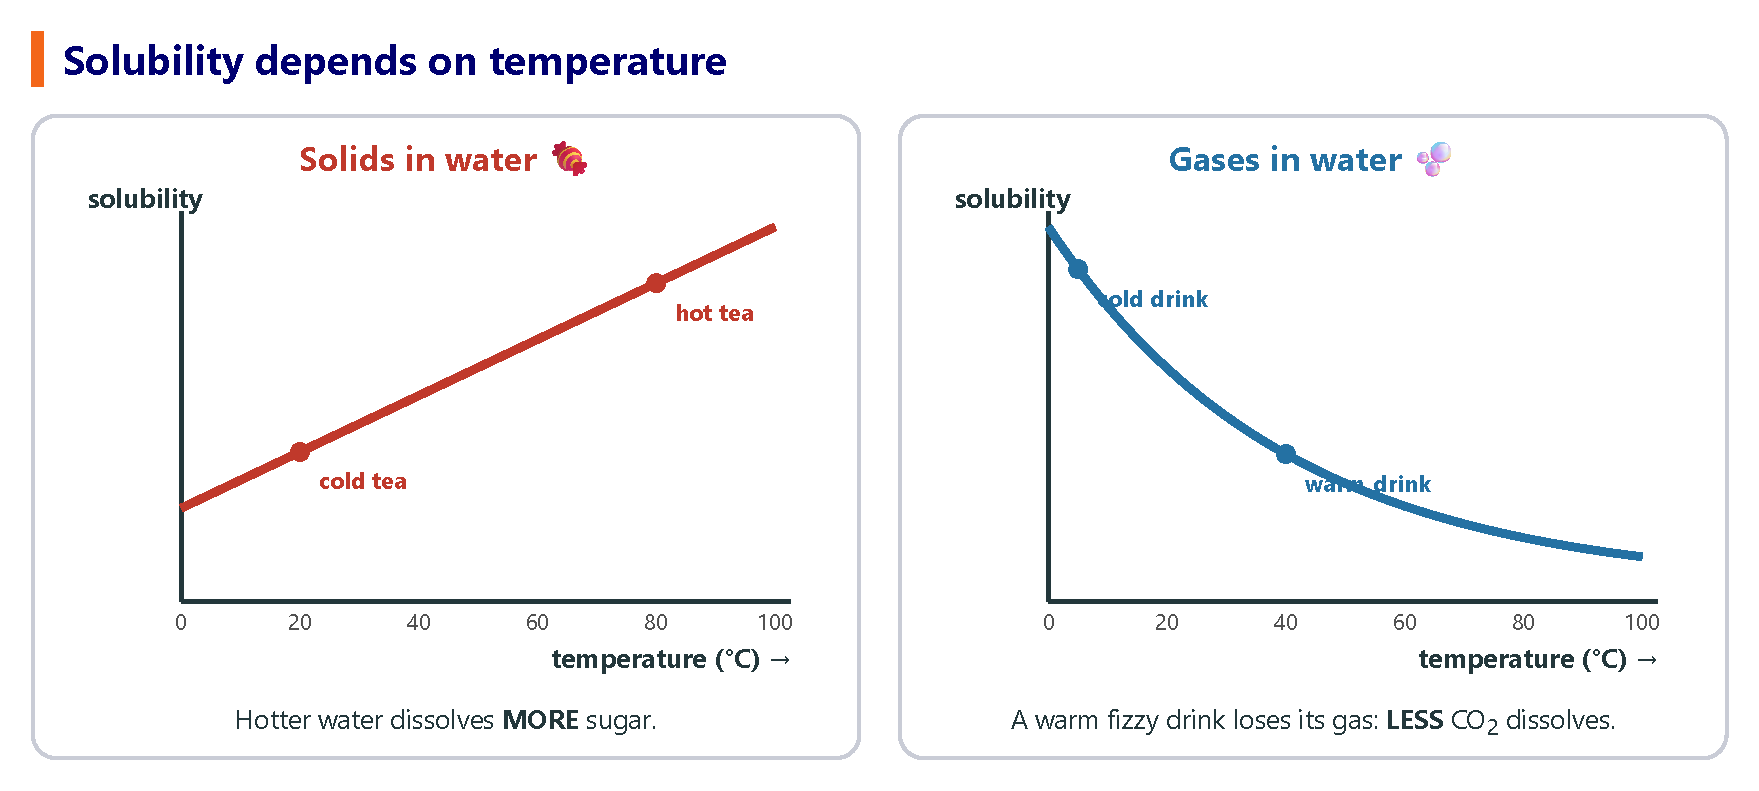
\includegraphics[width=\textwidth]{FigurasSVG/Unit_3_Diversity_of_Matter/pdf/solubility_graph.pdf}
%    \caption{La temperatura aumenta la solubilidad de la mayoría de los sólidos, pero disminuye la de los gases.}
%    \label{fig:u3_solubility_graph}
%\end{figure}

%\begin{impt}
%    La solubilidad depende de:
%    \begin{itemize}
%        \item \textbf{Las sustancias}: la sal y el azúcar se disuelven en agua; el aceite y la arena no.
%        \item \textbf{La temperatura}: mira las gráficas anteriores.
%        \item \textbf{Remover} \emph{no} cambia la solubilidad, pero hace que el soluto se disuelva \textbf{más deprisa}.
%    \end{itemize}
%\end{impt}

\begin{exercise}
    Se disuelven \qty{25}{\g} de azúcar en agua hasta obtener \qty{250}{\mL} de disolución. Calcula la concentración de la disolución en g/L.
    \begin{solu}
        \(V = \qty{250}{\mL} = \qty{0.250}{\litre}\); \quad \(C = \dfrac{\qty{25}{\g}}{\qty{0.250}{\litre}} = \qty{100}{\g\per\litre}\).
    \end{solu}
\end{exercise}

\begin{exercise}
    Se prepara una disolución disolviendo \qty{8}{\g} de sal en \qty{92}{\g} de agua.
    \begin{enumerate}[label=\letraminuscula]
        \item Calcula el porcentaje en masa de la disolución.
        \item Si tuviéramos \qty{500}{\g} de esta misma disolución, ¿qué masa de sal contendría?
    \end{enumerate}
    \begin{solu}
        \begin{enumerate}[label=\alph*)]
            \item Masa de disolución \(= \qty{8}{\g} + \qty{92}{\g} = \qty{100}{\g}\); \quad \(\% \text{ en masa} = \dfrac{\qty{8}{\g}}{\qty{100}{\g}} \cdot 100 = \qty{8}{\percent}\).
            \item \(\qty{500}{\g} \cdot \dfrac{8}{100} = \qty{40}{\g}\) de sal.
        \end{enumerate}
    \end{solu}
\end{exercise}

\begin{exercise}
    Explica, usando la idea de solubilidad, por qué el azúcar se disuelve mejor en el té caliente que en el té frío, y por qué una lata de refresco pierde antes las burbujas si se deja abierta en un día caluroso.
    \begin{solu}
        La solubilidad de un sólido como el azúcar \textbf{aumenta} con la temperatura, así que en el té caliente se disuelve más azúcar. \\
        La solubilidad de un gas como el \ch{CO2} \textbf{disminuye} con la temperatura: al calentarse el refresco, cabe menos gas disuelto, y el gas se escapa en forma de burbujas.
    \end{solu}
\end{exercise}

\begin{exercise}
    Una botella contiene \qty{750}{\mL} de una disolución de concentración \qty{40}{\g\per\litre}. Calcula la masa de soluto disuelta en la botella.
    \begin{solu}
        \(\text{masa} = C \cdot V = \qty{40}{\g\per\litre} \cdot \qty{0.750}{\litre} = \qty{30}{\g}\) de soluto.
    \end{solu}
\end{exercise}

\begin{exercise}
    Se prepara una disolución disolviendo \qty{12}{\g} de sal en el agua necesaria para obtener \qty{200}{\g} de disolución.
    \begin{enumerate}[label=\letraminuscula]
        \item Calcula el porcentaje en masa de la disolución.
        \item ¿Qué masa de esta disolución necesitarías para tener \qty{6}{\g} de sal?
    \end{enumerate}
    \begin{solu}
        \begin{enumerate}[label=\alph*)]
            \item \(\% \text{ en masa} = \dfrac{\qty{12}{\g}}{\qty{200}{\g}} \cdot 100 = \qty{6}{\percent}\).
            \item \(\qty{6}{\g} \cdot \dfrac{100}{6} = \qty{100}{\g}\) de disolución.
        \end{enumerate}
    \end{solu}
\end{exercise}

\subsection{Mezclas heterogéneas}

\begin{definition}[Mezcla heterogénea]
    Es una mezcla cuyos componentes \textbf{se pueden distinguir a simple vista}: vemos partes diferentes, y dos muestras tomadas en sitios distintos pueden tener una composición diferente.
\end{definition}

\begin{example}
    Algunas mezclas heterogéneas:
    \begin{itemize}
        \item El \textbf{granito}: se ven granos de tres minerales distintos (blancos, negros y rosados o grises).
        \item La \textbf{arena con agua} o el \textbf{agua con barro}: se ve la arena o el barro, que se deposita en el fondo.
        \item El \textbf{aceite con agua}: dos capas, con el aceite arriba.
        \item Una \textbf{ensalada}, una \textbf{paella} o una \textbf{pizza}: se reconoce cada ingrediente.
    \end{itemize}
\end{example}

Algunas mezclas heterogéneas son especiales: sus componentes son tan pequeños que, a simple vista, la mezcla \textbf{parece} homogénea, y necesitamos un microscopio para ver sus distintas partes. Son los \textbf{coloides}.

\subsubsection{Coloides}

\begin{definition}[Coloide]
    Es una mezcla heterogénea que a simple vista \textbf{parece} homogénea, pero en la que al microscopio se ven partículas de distinta composición. Ejemplos: la leche, la sangre, la mayonesa, la gelatina, la niebla.
\end{definition}

\begin{definition}[Efecto Tyndall]
    Es la dispersión de la luz por las partículas de un coloide, que hace visible un haz de luz en su interior. Las disoluciones \textbf{no} presentan este efecto.
\end{definition}

\begin{figure}[H]
    \centering
    % [FIGURA ORIGINAL] \includegraphics[width=\textwidth]{Unit_3/tyndall}
    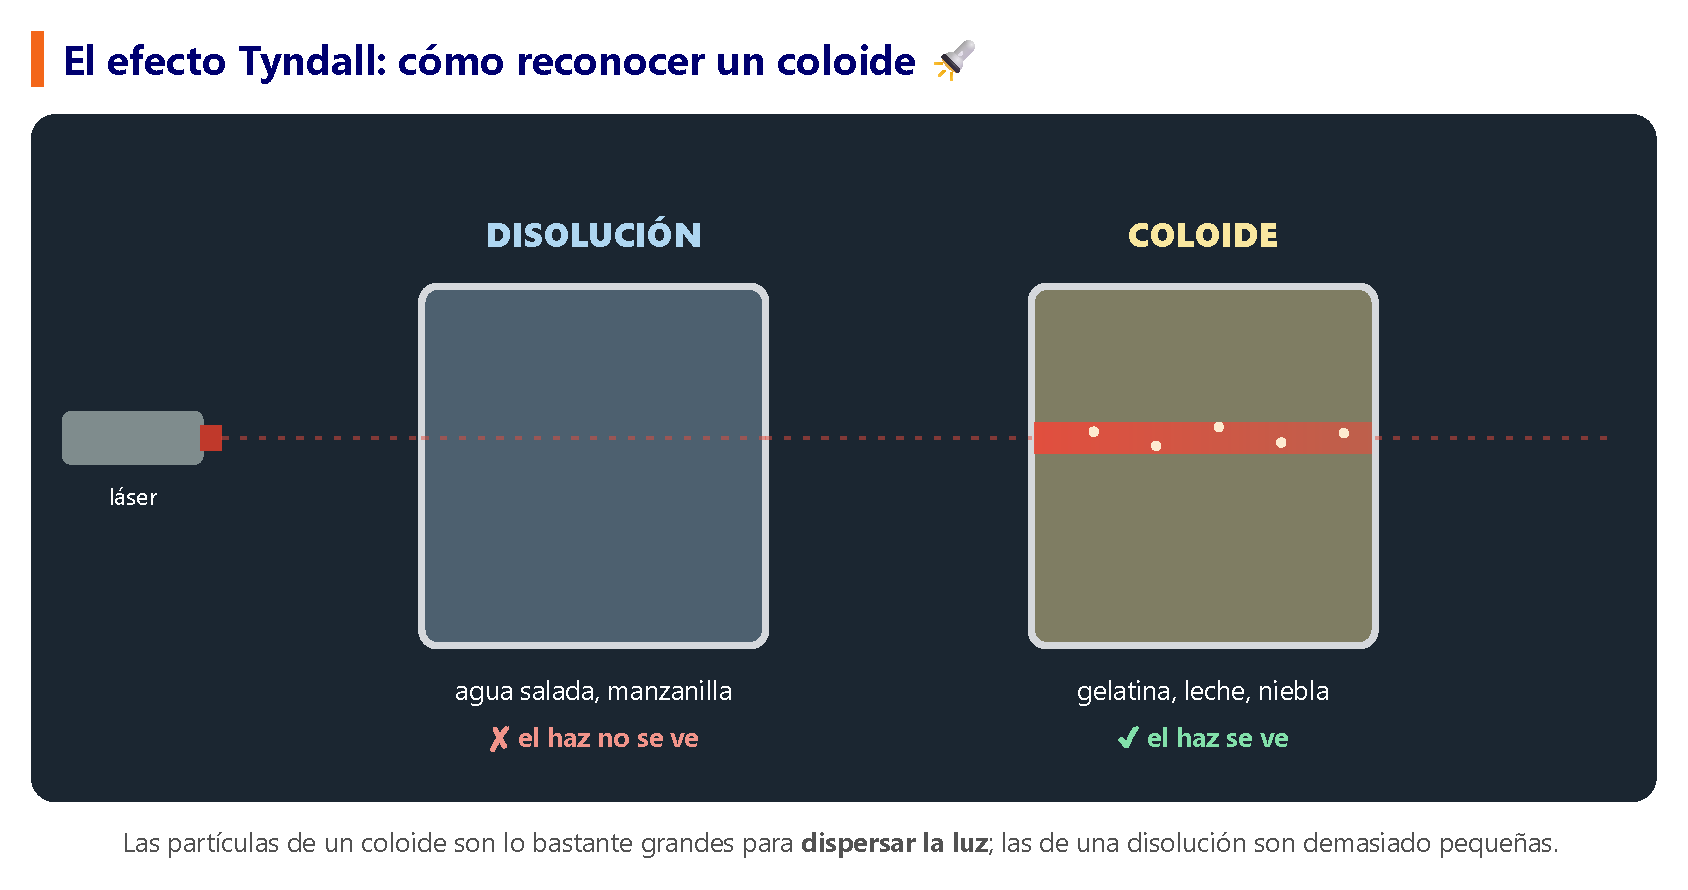
\includegraphics[width=\textwidth]{FigurasSVG/Unit_3_Diversity_of_Matter/pdf/tyndall_es.pdf}
    \caption{El efecto Tyndall permite distinguir un coloide de una disolución.}
    \label{fig:u3_tyndall}
\end{figure}

\begin{didyouknow}
    Cuando los rayos de sol atraviesan los árboles en una mañana de niebla, o entran por la ventana de una habitación con polvo, ¡estás viendo el efecto Tyndall! La niebla y el aire con polvo son coloides, y sus partículas dispersan la luz del sol.
\end{didyouknow}

\begin{exercise}
    Explica por qué una disolución de sulfato de cobre en agua no presenta efecto Tyndall y, en cambio, una mezcla de gelatina en agua sí.
    \begin{solu}
        En la disolución de sulfato de cobre las partículas disueltas son pequeñísimas, demasiado pequeñas para dispersar la luz, así que el haz no se ve. En la gelatina las partículas son más grandes (de tamaño coloidal) y dispersan la luz, así que el haz se ve: es el \textbf{efecto Tyndall}.
    \end{solu}
\end{exercise}

\begin{exercise}
    Clasifica cada mezcla como \textbf{disolución} o \textbf{coloide}, dando una razón basada en el tamaño de las partículas: mayonesa, agua de mar, nata montada, vinagre.
    \begin{solu}
        Mayonesa: \textbf{coloide} (gotitas de aceite dispersas en agua). \\
        Agua de mar: \textbf{disolución} (sales disueltas, partículas muy pequeñas). \\
        Nata montada: \textbf{coloide} (burbujitas de aire y gotitas de grasa). \\
        Vinagre: \textbf{disolución} (ácido acético disuelto en agua).
    \end{solu}
\end{exercise}

\subsubsection{Emulsiones}

\begin{definition}[Emulsión]
    Es un coloide formado por dos líquidos que no se mezclan (como el aceite y el agua), que se mantienen unidos gracias a una tercera sustancia llamada \textbf{emulsionante}.
\end{definition}

\begin{figure}[H]
    \centering
    % [FIGURA ORIGINAL] \includegraphics[width=\textwidth]{Unit_3/emulsion}
    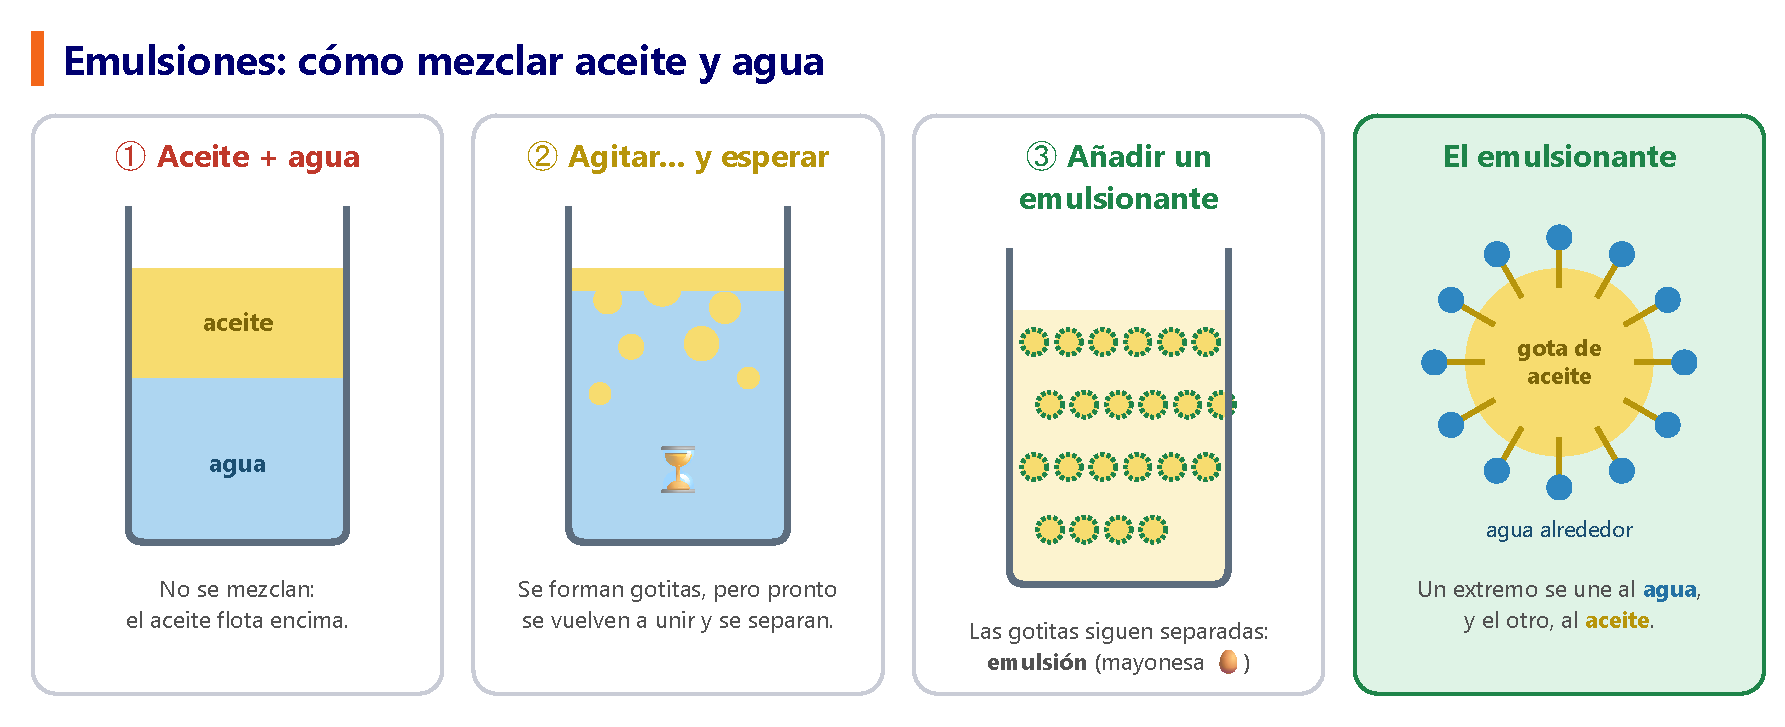
\includegraphics[width=\textwidth]{FigurasSVG/Unit_3_Diversity_of_Matter/pdf/emulsion_es.pdf}
    \caption{Un emulsionante mantiene separadas las gotitas de aceite dentro del agua.}
    \label{fig:u3_emulsion}
\end{figure}

\begin{example}
    En la mayonesa el emulsionante es la \textbf{lecitina} de la yema de huevo; en la leche es la \textbf{caseína}, una proteína de la leche. El jabón también actúa como emulsionante: por eso quita la grasa de las manos.
\end{example}

\begin{exercise}
    Explica qué ocurre si agitas una mezcla de aceite y agua \textbf{sin} añadir ningún emulsionante, y por qué.
    \begin{solu}
        Al agitar, el aceite se rompe en gotitas, pero sin emulsionante nada las mantiene separadas. Las gotitas se vuelven a unir y la mezcla se separa en dos capas, con el aceite, menos denso, arriba.
    \end{solu}
\end{exercise}

\begin{exercise}
    Identifica el emulsionante de cada emulsión: a) la mayonesa; b) la leche; c) muchas cremas cosméticas.
    \begin{solu}
        \begin{enumerate}[label=\alph*)]
            \item La lecitina de la yema de huevo.
            \item La caseína, una proteína de la leche.
            \item Ceras emulsionantes o moléculas parecidas al jabón, con un extremo que se mezcla con el agua y otro con el aceite.
        \end{enumerate}
    \end{solu}
\end{exercise}

\subsection{Tamaño de las partículas y tipos de mezclas}

\begin{figure}[H]
    \centering
    % [FIGURA ORIGINAL] \includegraphics[width=\textwidth]{Unit_3/particle_size}
    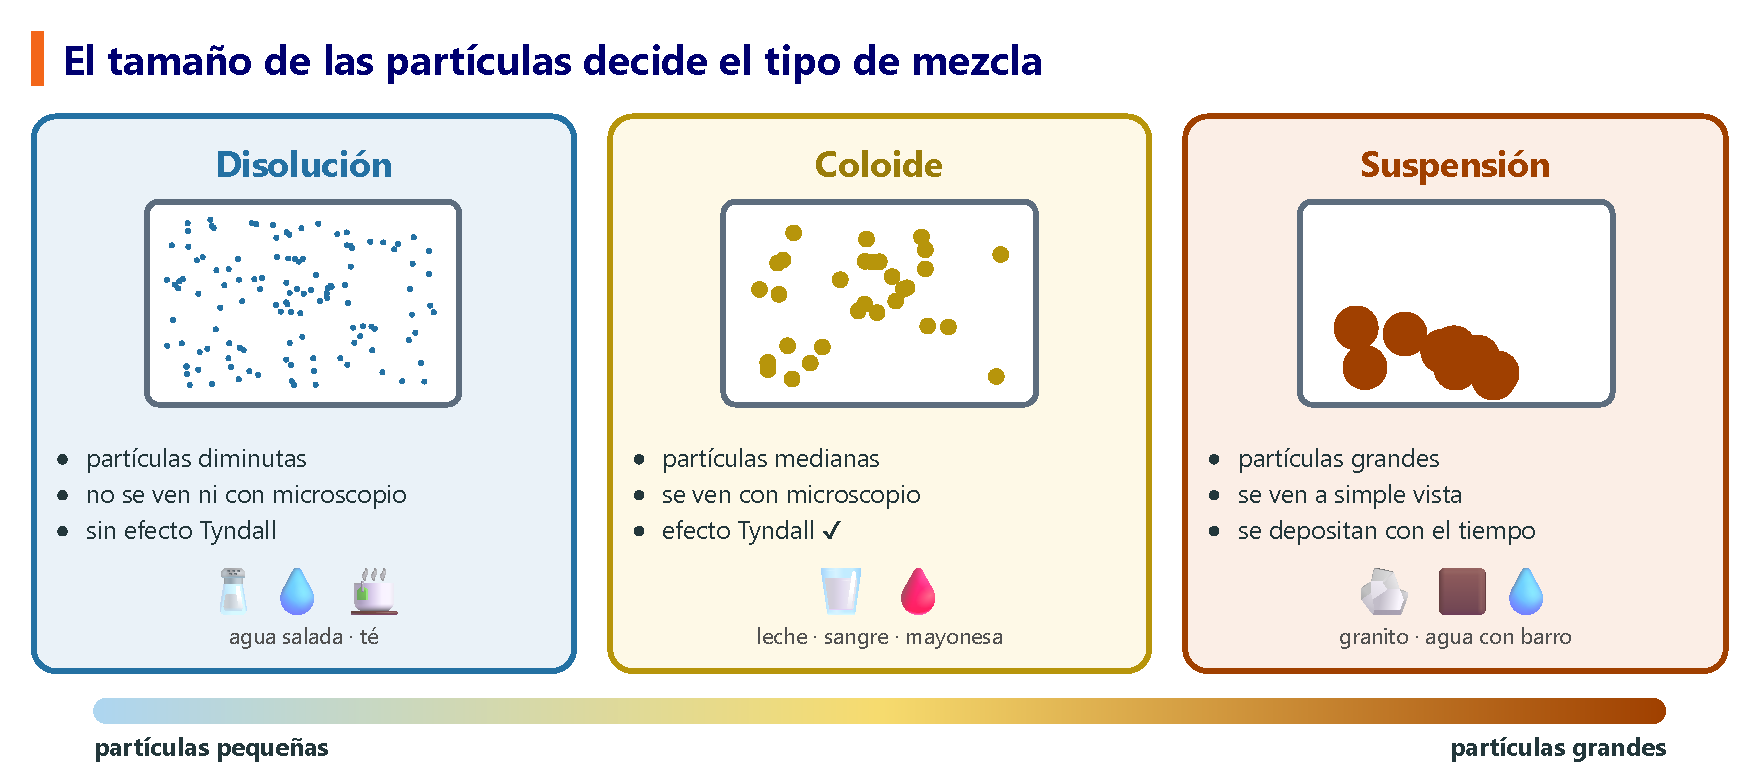
\includegraphics[width=\textwidth]{FigurasSVG/Unit_3_Diversity_of_Matter/pdf/particle_size_es.pdf}
    \caption{Cuanto más grandes son las partículas dispersas, más heterogénea es la mezcla.}
    \label{fig:u3_particle_size}
\end{figure}

\begin{exercise}
    Clasifica estas mezclas como homogéneas o heterogéneas, e indica si son coloides: merengue, suero fisiológico, monedas (aleación metálica), mármol, leche, refrescos con gas.
    \begin{solu}
        Merengue: \textbf{heterogénea}, coloide (aire atrapado en la clara de huevo). \\
        Suero fisiológico: \textbf{homogénea} (una disolución). \\
        Monedas: \textbf{homogénea} (una aleación, una disolución sólida). \\
        Mármol: \textbf{heterogénea} (se ven vetas y granos). \\
        Leche: \textbf{heterogénea}, coloide, aunque parezca homogénea. \\
        Refrescos con gas: \textbf{homogénea} (una disolución de \ch{CO2} en agua).
    \end{solu}
\end{exercise}

\begin{exercise}
    Ordena estos tres sistemas de \textbf{menor} a \textbf{mayor} tamaño de las partículas dispersas, e indica qué tipo de mezcla es cada uno: disolución de azúcar, agua de río con barro, leche.
    \begin{solu}
        \textbf{Disolución de azúcar} (disolución) \(<\) \textbf{leche} (coloide) \(<\) \textbf{agua de río con barro} (suspensión).
    \end{solu}
\end{exercise}

%----------------------------------------------------------------------------------------

\section{De qué está formada la materia}

\begin{definition}[Átomo]
    Es la partícula diminuta que forma toda la materia. Los átomos están formados por partículas aún más pequeñas: \textbf{protones}, \textbf{neutrones} y \textbf{electrones}.
\end{definition}

Los científicos no podían ver los átomos, así que imaginaron \textbf{modelos} para explicar los resultados de sus experimentos. Cada experimento nuevo mejoraba el modelo:

\begin{figure}[H]
    \centering
    % [FIGURA ORIGINAL] \includegraphics[width=\textwidth]{Unit_3/atomic_models}
    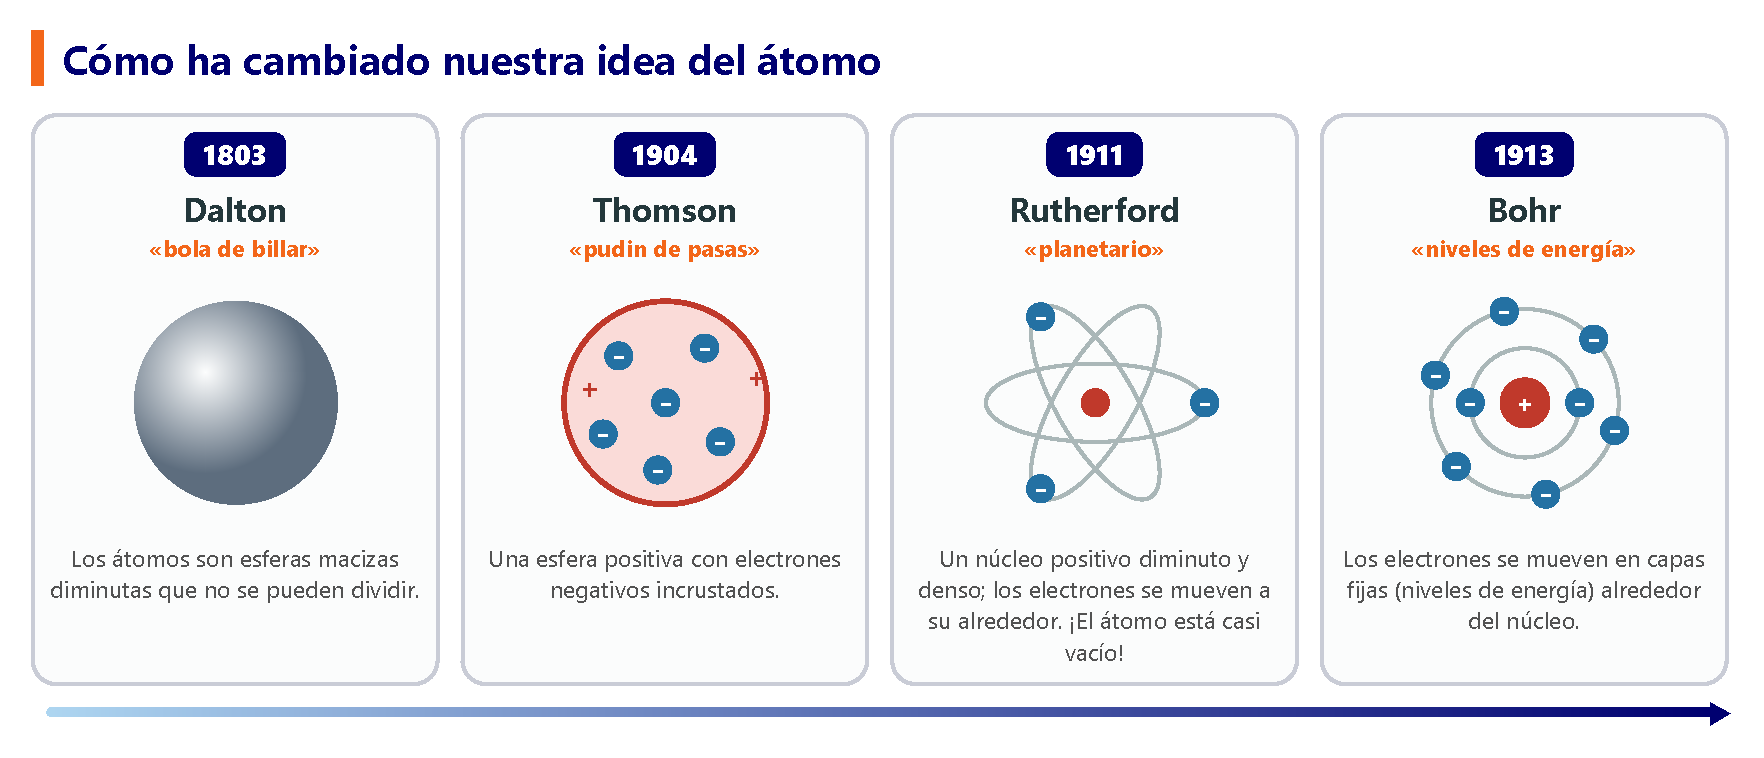
\includegraphics[width=\textwidth]{FigurasSVG/Unit_3_Diversity_of_Matter/pdf/atomic_models_es.pdf}
    \caption{Los principales modelos atómicos.}
    \label{fig:u3_atomic_models}
\end{figure}

\begin{didyouknow}
    ¡El átomo está casi completamente vacío! Si el núcleo fuera del tamaño de un balón de fútbol en el centro de un estadio, los electrones serían como granitos de arena moviéndose por las últimas filas de las gradas. Rutherford lo descubrió en 1911, cuando lanzó partículas contra una lámina de oro muy fina y casi todas la atravesaron sin desviarse.
\end{didyouknow}

\subsection{La estructura del átomo}

\begin{figure}[H]
    \centering
    % [FIGURA ORIGINAL] \includegraphics[width=\textwidth]{Unit_3/atom_structure}
    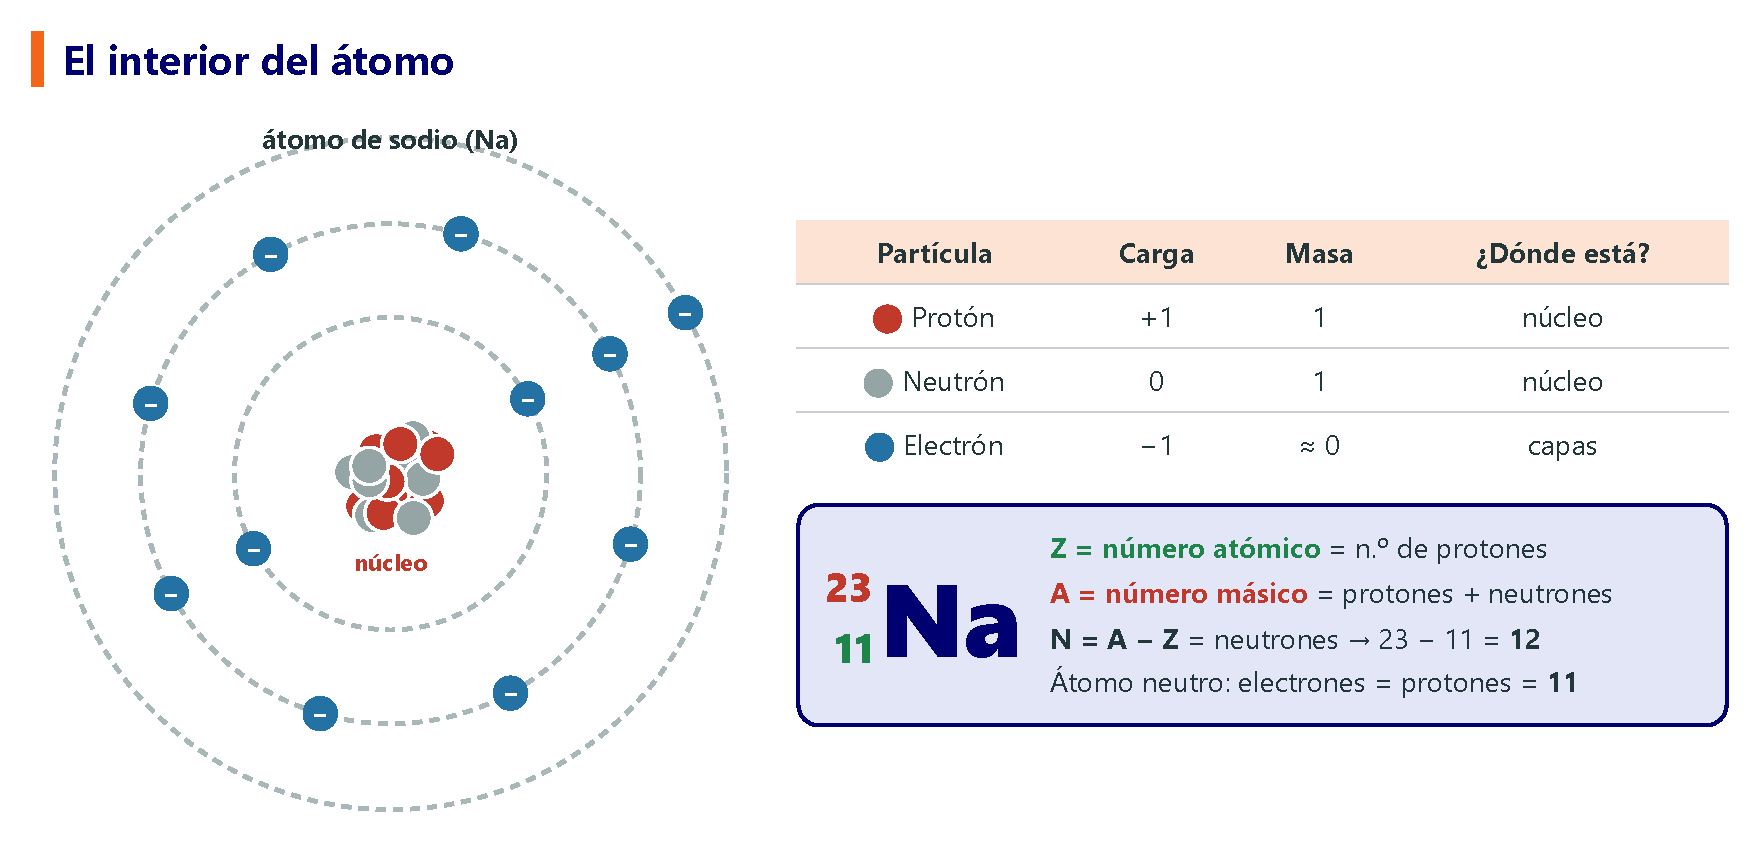
\includegraphics[width=\textwidth]{FigurasSVG/Unit_3_Diversity_of_Matter/pdf/atom_structure_es.pdf}
    \caption{Las partículas del átomo y cómo se representa un átomo.}
    \label{fig:u3_atom_structure}
\end{figure}

\begin{impt}
    Casi toda la \textbf{masa} del átomo está en el \textbf{núcleo}; casi todo su \textbf{volumen} es el espacio por el que se mueven los electrones. En un átomo \textbf{neutro}, el número de electrones \(=\) número de protones.
\end{impt}

\begin{definition}[Número atómico \(Z\) y número másico \(A\)]
    \(Z\) es el número de \textbf{protones}: nos dice de qué elemento es el átomo. \(A\) es el número de protones \textbf{más} neutrones. Por tanto, el número de neutrones es
    \begin{equation*}
        N = A - Z
    \end{equation*}
\end{definition}

\begin{example}
    Sodio, \ch{^{23}_{11}Na}: \(Z = 11\) y \(A = 23\). Tiene 11 protones, 11 electrones (es neutro) y \(N = 23 - 11 = 12\) neutrones.
\end{example}

\begin{definition}[Isótopos]
    Son átomos del \textbf{mismo} elemento (mismo \(Z\)) con \textbf{distinto} número de neutrones (distinto \(A\)).
\end{definition}

\begin{figure}[H]
    \centering
    % [FIGURA ORIGINAL] \includegraphics[width=0.9\textwidth]{Unit_3/isotopes}
    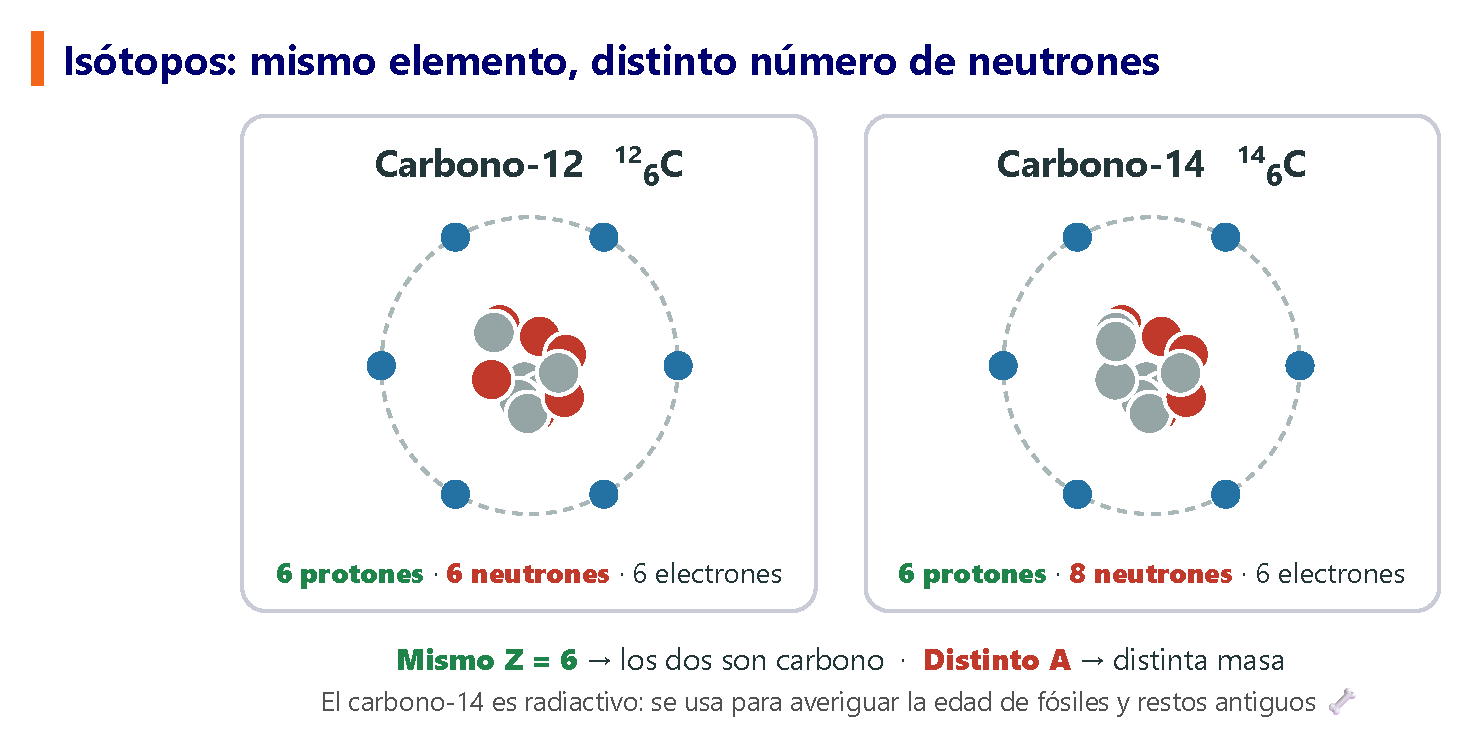
\includegraphics[width=0.9\textwidth]{FigurasSVG/Unit_3_Diversity_of_Matter/pdf/isotopes_es.pdf}
    \caption{Dos isótopos del carbono.}
    \label{fig:u3_isotopes}
\end{figure}

\begin{exercise}
    Un átomo tiene 17 protones, 17 electrones y 18 neutrones.
    \begin{enumerate}[label=\letraminuscula]
        \item Indica su número atómico \(Z\) y su número másico \(A\).
        \item ¿Qué elemento químico es? (Pista: el número atómico 17 es el cloro.)
    \end{enumerate}
    \begin{solu}
        \begin{enumerate}[label=\alph*)]
            \item \(Z = 17\); \(A = 17 + 18 = 35\).
            \item \textbf{Cloro}, \ch{Cl}.
        \end{enumerate}
    \end{solu}
\end{exercise}

\begin{exercise}
    Dos isótopos de un elemento tienen números másicos 35 y 37, y los dos tienen \(Z = 17\). Explica qué tienen en común y en qué se diferencian.
    \begin{solu}
        Los dos tienen 17 protones y 17 electrones (son el mismo elemento). Tienen distinto número de neutrones: \(N = 35 - 17 = 18\) y \(N = 37 - 17 = 20\).
    \end{solu}
\end{exercise}

\begin{exercise}
    Completa la tabla para estos átomos neutros:
    \begin{center}
        \renewcommand{\arraystretch}{1.3}
        \begin{tabular}{cccccc}
            \toprule
            \textbf{Elemento} & \(Z\) & \(A\) & \textbf{Protones} & \textbf{Neutrones} & \textbf{Electrones} \\
            \midrule
            Oxígeno & 8 & 16 & & & \\
            Magnesio & 12 & 24 & & & \\
            Potasio & 19 & 39 & & & \\
            \bottomrule
        \end{tabular}
    \end{center}
    \begin{solu}
        Oxígeno: 8 protones, \(16 - 8 = 8\) neutrones, 8 electrones. \\
        Magnesio: 12 protones, \(24 - 12 = 12\) neutrones, 12 electrones. \\
        Potasio: 19 protones, \(39 - 19 = 20\) neutrones, 19 electrones.
    \end{solu}
\end{exercise}

\begin{exercise}
    El potasio-40 (\(Z = 19\), \(A = 40\)) y el calcio-40 (\(Z = 20\), \(A = 40\)) tienen el mismo número másico. Explica por qué \textbf{no} son isótopos y calcula el número de neutrones de cada átomo.
    \begin{solu}
        Los isótopos tienen que tener el \textbf{mismo} \(Z\). Aquí \(Z\) es distinto (19 y 20), así que son elementos diferentes. \\
        Neutrones: potasio-40, \(N = 40 - 19 = 21\); calcio-40, \(N = 40 - 20 = 20\).
    \end{solu}
\end{exercise}

\subsection{Elementos, moléculas y cristales}

\begin{definition}[Elemento químico]
    Es el conjunto de todos los átomos que tienen el mismo número de protones (\(Z\)). Se conocen 118 elementos, ordenados en la tabla periódica.
\end{definition}

\begin{figure}[H]
    \centering
    % [FIGURA ORIGINAL] \includegraphics[width=\textwidth]{Unit_3/particle_arrangements}
    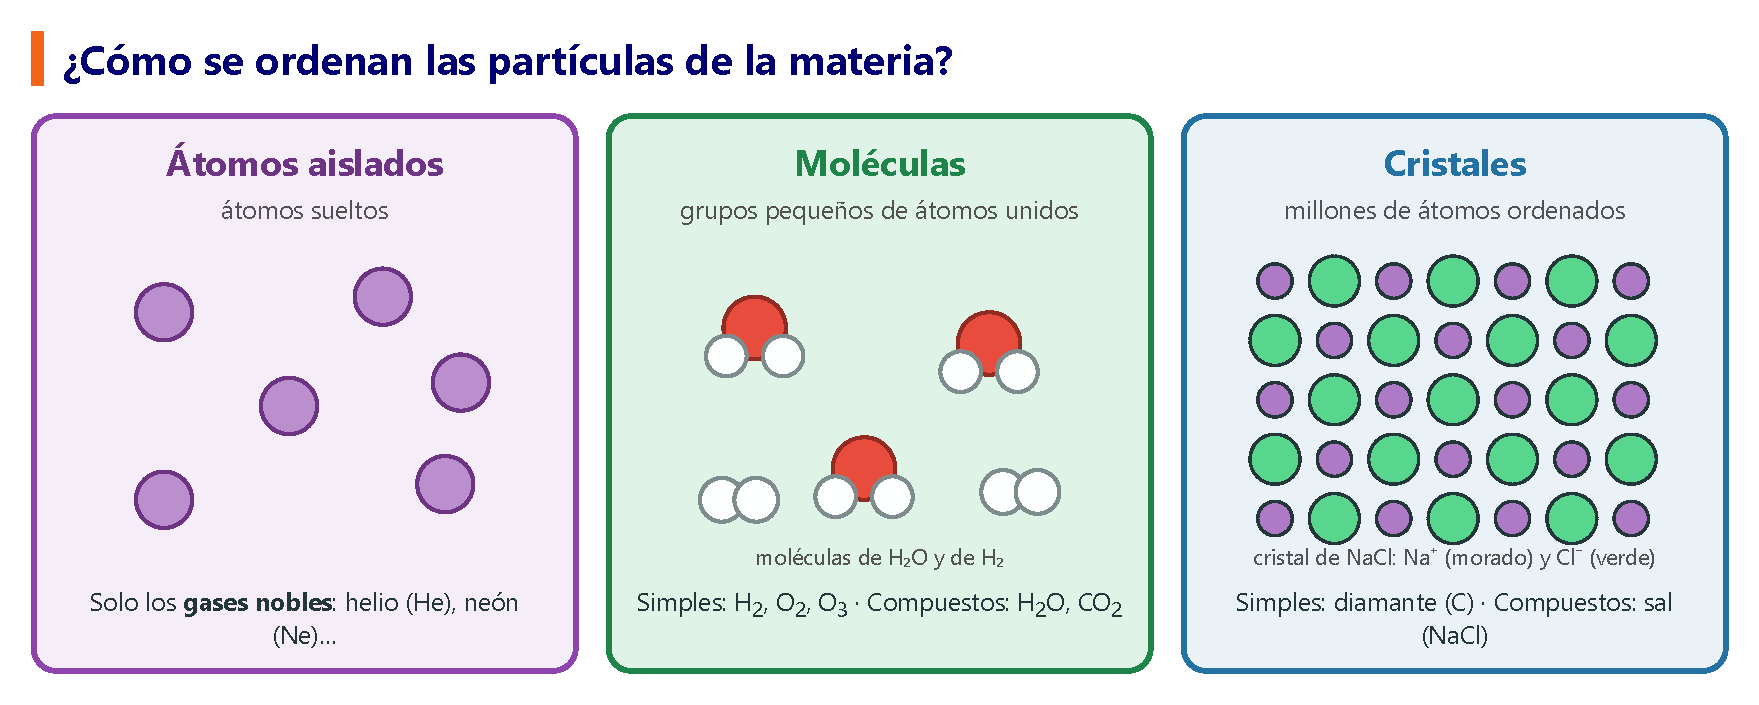
\includegraphics[width=\textwidth]{FigurasSVG/Unit_3_Diversity_of_Matter/pdf/particle_arrangements_es.pdf}
    \caption{Las tres formas en que pueden estar organizadas las partículas de una sustancia.}
    \label{fig:u3_particle_arrangements}
\end{figure}

\begin{impt}
    \negsubro{Mezcla o compuesto}: el hidrógeno gaseoso (\ch{H2}) y el oxígeno gaseoso (\ch{O2}) se pueden mezclar en \textbf{cualquier} proporción: eso es una mezcla. En el agua (\ch{H2O}) hay \textbf{siempre} 2 átomos de hidrógeno por cada átomo de oxígeno: eso es un compuesto, y sus propiedades son completamente distintas de las de los dos gases.
\end{impt}

\begin{exercise}
    Observa las tres cajas de la figura siguiente.
    \begin{figure}[H]
        \centering
        % [FIGURA ORIGINAL] \includegraphics[width=0.95\textwidth]{Unit_3/substances_particles}
        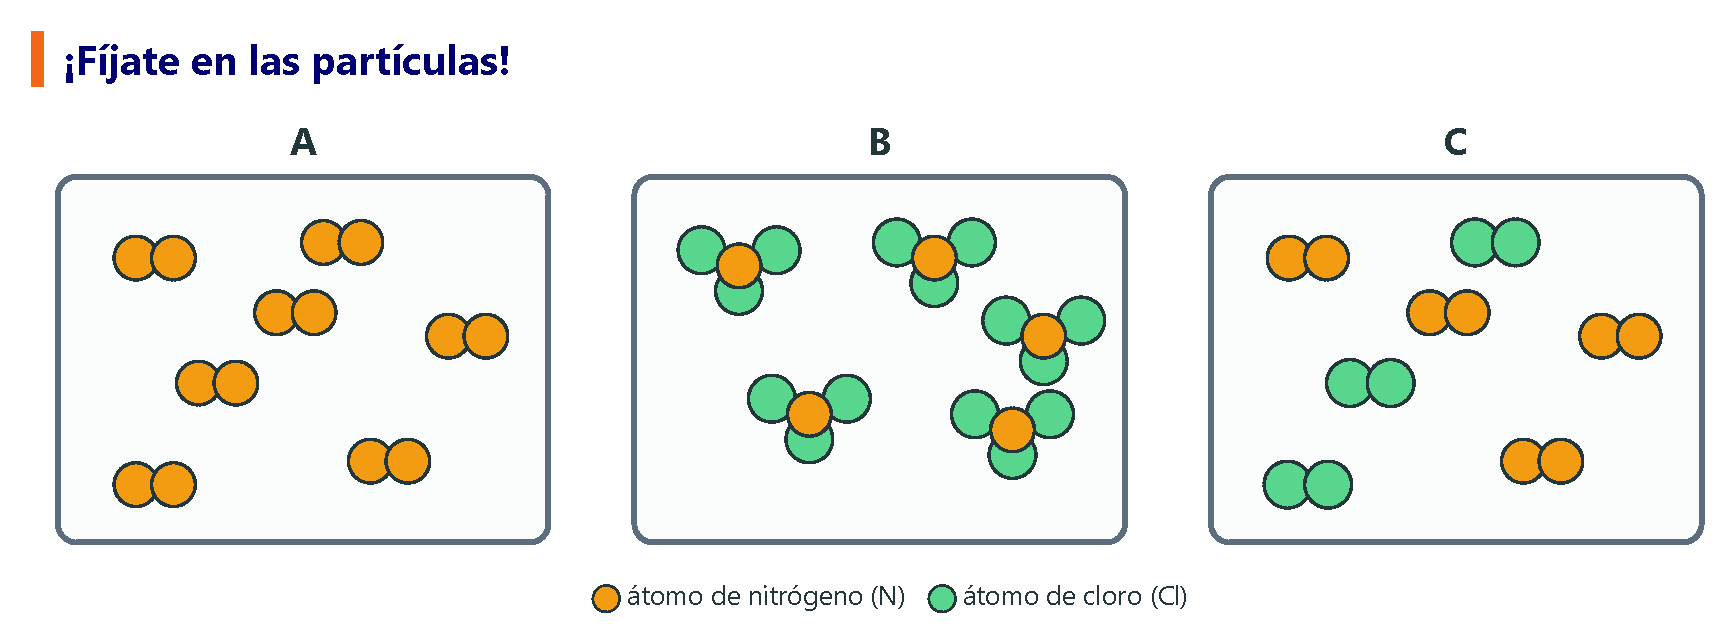
\includegraphics[width=0.95\textwidth]{FigurasSVG/Unit_3_Diversity_of_Matter/pdf/substances_particles_es.pdf}
    \end{figure}
    ¿Qué caja representa: a) una sustancia simple; b) un compuesto; c) una mezcla? Explica cómo lo sabes.
    \begin{solu}
        \begin{enumerate}[label=\alph*)]
            \item \textbf{A}: todas las moléculas son iguales (\ch{N2}) y están formadas por un solo tipo de átomo.
            \item \textbf{B}: todas las moléculas son iguales (\ch{NCl3}), pero cada una tiene dos tipos de átomos.
            \item \textbf{C}: hay dos tipos de moléculas distintas (\ch{N2} y \ch{Cl2}).
        \end{enumerate}
    \end{solu}
\end{exercise}

\begin{exercise}
    Clasifica como sustancia simple o compuesto, y como formada por moléculas o por un cristal: diamante (\ch{C}), cloruro de sodio (\ch{NaCl}), hidrógeno gaseoso (\ch{H2}), agua (\ch{H2O}).
    \begin{solu}
        Diamante: sustancia simple, cristal. \\
        Cloruro de sodio: compuesto, cristal. \\
        Hidrógeno gaseoso: sustancia simple, moléculas. \\
        Agua: compuesto, moléculas.
    \end{solu}
\end{exercise}

\begin{exercise}
    Indica si cada una de estas sustancias está formada por \textbf{átomos aislados}, \textbf{moléculas} o un \textbf{cristal}: neón gaseoso (\ch{Ne}); dióxido de carbono gaseoso (\ch{CO2}); un diamante (\ch{C}); sal común (\ch{NaCl}).
    \begin{solu}
        Neón: \textbf{átomos aislados} (gas noble). Dióxido de carbono: \textbf{moléculas}. Diamante: \textbf{cristal}. Sal común: \textbf{cristal}.
    \end{solu}
\end{exercise}

%----------------------------------------------------------------------------------------

\section{La tabla periódica de los elementos}

\begin{definition}[Tabla periódica]
    Es una tabla con los 118 elementos conocidos, ordenados de menor a mayor \textbf{número atómico} \(Z\). Las filas se llaman \negsubro{periodos} (7) y las columnas \negsubro{grupos} (18).
\end{definition}

\begin{figure}[H]
    \centering
    % [FIGURA ORIGINAL] \includegraphics[width=\textwidth]{Unit_3/periodic_table}
    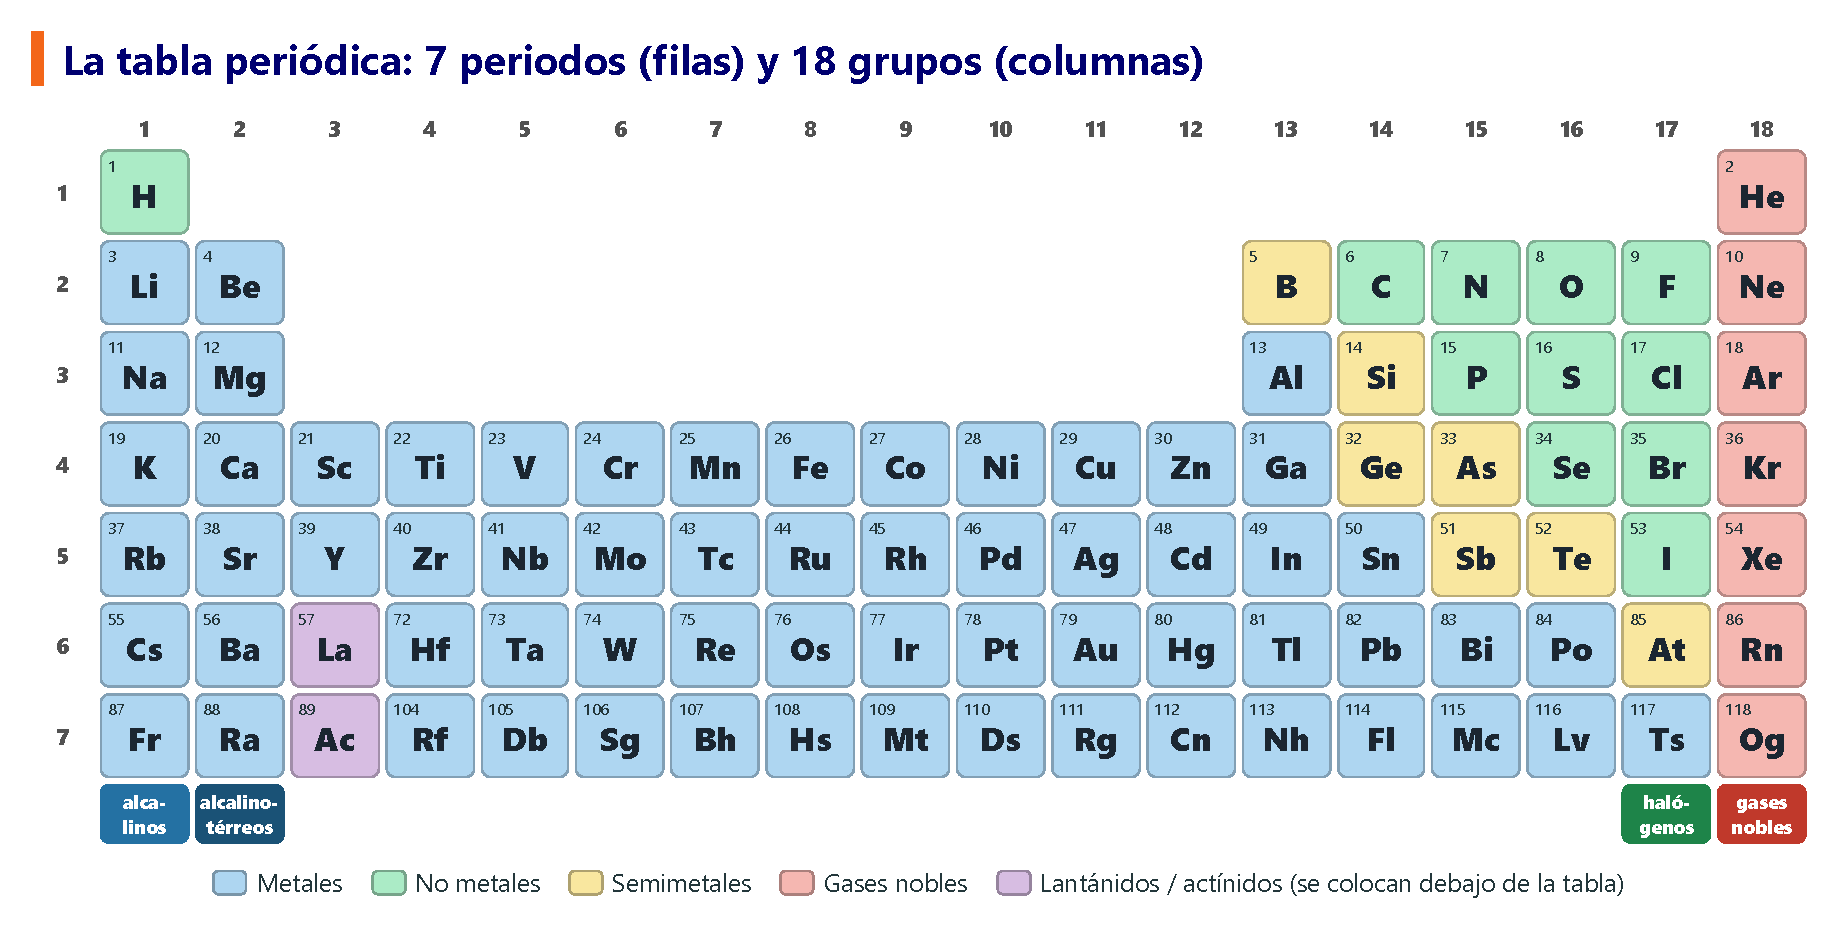
\includegraphics[width=\textwidth]{FigurasSVG/Unit_3_Diversity_of_Matter/pdf/periodic_table_es.pdf}
    \caption{La tabla periódica: metales, no metales, semimetales y gases nobles.}
    \label{fig:u3_periodic_table}
\end{figure}

\begin{impt}
    \begin{itemize}
        \item Cada elemento tiene un \textbf{símbolo}: la primera letra siempre es mayúscula y la segunda (si la hay), minúscula: \ch{H}, \ch{Ca}, \ch{Cl}.
        \item Los elementos de un mismo \textbf{grupo} tienen \textbf{propiedades parecidas}.
        \item El número del \textbf{periodo} nos dice cuántas capas de electrones tienen los átomos.
    \end{itemize}
\end{impt}

\begin{table}[H]
    \centering
    \small
    \renewcommand{\arraystretch}{1.35}
    \begin{tabular}{lp{9.5cm}}
        \toprule
        \textbf{Tipo} & \textbf{Propiedades} \\
        \midrule
        Metales & La mayoría de los elementos. Brillantes, sólidos a temperatura ambiente (excepto el mercurio), buenos conductores del calor y de la electricidad. \\
        No metales & Malos conductores; muchos son gases (\ch{O2}, \ch{N2}) o sólidos frágiles (\ch{S}, \ch{C}). \\
        Semimetales & Propiedades intermedias (el silicio, que se usa en los chips de los ordenadores). \\
        Gases nobles & Grupo 18. Muy estables: casi nunca reaccionan. \\
        \bottomrule
    \end{tabular}
    \caption{Tipos de elementos de la tabla periódica.}
    \label{tab:u3_element_types}
\end{table}

\begin{didyouknow}
    Dmitri Mendeléiev organizó la primera tabla periódica en 1869. Dejó huecos vacíos para elementos que todavía no se habían descubierto, e incluso predijo sus propiedades. Años después se descubrieron el galio y el germanio\ldots{} ¡y encajaban perfectamente!
\end{didyouknow}

\begin{exercise}
    Usa la tabla periódica para indicar el nombre y el símbolo de: el elemento de número atómico 6; el elemento de número atómico 17; el gas noble del periodo 2.
    \begin{solu}
        \(Z = 6\): \textbf{carbono}, \ch{C}. \quad \(Z = 17\): \textbf{cloro}, \ch{Cl}. \quad Gas noble del periodo 2: \textbf{neón}, \ch{Ne}.
    \end{solu}
\end{exercise}

\begin{exercise}
    Indica si cada elemento es un metal, un no metal, un semimetal o un gas noble: sodio (\ch{Na}), oxígeno (\ch{O}), silicio (\ch{Si}), argón (\ch{Ar}), hierro (\ch{Fe}).
    \begin{solu}
        Sodio: metal. Oxígeno: no metal. Silicio: semimetal. Argón: gas noble. Hierro: metal.
    \end{solu}
\end{exercise}

\begin{exercise}
    Los elementos X, Y y Z están en el mismo \textbf{periodo}, pero en grupos distintos. ¿Qué te dice esto sobre el número de capas de electrones de sus átomos? ¿Son el mismo elemento?
    \begin{solu}
        Tienen el \textbf{mismo número de capas de electrones} (igual al número del periodo). \textbf{No} son el mismo elemento: al estar en grupos distintos, tienen números atómicos distintos.
    \end{solu}
\end{exercise}

\subsection{Algunos grupos importantes}

\begin{table}[H]
    \centering
    \small
    \renewcommand{\arraystretch}{1.35}
    \begin{tabular}{lcp{7.5cm}}
        \toprule
        \textbf{Nombre} & \textbf{Grupo} & \textbf{Ejemplos y propiedades} \\
        \midrule
        Alcalinos & 1 & \ch{Li}, \ch{Na}, \ch{K}: metales muy reactivos (reaccionan violentamente con el agua). \\
        Alcalinotérreos & 2 & \ch{Mg}, \ch{Ca}: metales reactivos. \\
        Halógenos & 17 & \ch{F}, \ch{Cl}, \ch{Br}, \ch{I}: no metales muy reactivos. \\
        Gases nobles & 18 & \ch{He}, \ch{Ne}, \ch{Ar}: gases muy poco reactivos. \\
        \bottomrule
    \end{tabular}
    \caption{Algunos grupos importantes de la tabla periódica.}
    \label{tab:u3_groups}
\end{table}

\begin{exercise}
    Indica el grupo al que pertenece cada elemento y si será muy reactivo o muy poco reactivo: potasio (\ch{K}), neón (\ch{Ne}), cloro (\ch{Cl}).
    \begin{solu}
        Potasio: \textbf{alcalino} (grupo 1), muy reactivo. \\
        Neón: \textbf{gas noble} (grupo 18), muy poco reactivo. \\
        Cloro: \textbf{halógeno} (grupo 17), muy reactivo.
    \end{solu}
\end{exercise}

\begin{exercise}
    El sodio (\ch{Na}) y el potasio (\ch{K}) pertenecen los dos al grupo 1. Predice si reaccionan con el agua de forma parecida y explica por qué.
    \begin{solu}
        Sí. Los elementos de un mismo grupo tienen propiedades químicas parecidas. Los dos son \textbf{alcalinos}, así que los dos reaccionan vivamente con el agua, desprendiendo hidrógeno gaseoso y formando un hidróxido del metal.
    \end{solu}
\end{exercise}

\begin{exercise}
    Clasifica cada elemento como alcalino, alcalinotérreo, halógeno o gas noble: litio (\ch{Li}), flúor (\ch{F}), calcio (\ch{Ca}), criptón (\ch{Kr}), bromo (\ch{Br}).
    \begin{solu}
        Litio: alcalino. Flúor: halógeno. Calcio: alcalinotérreo. Criptón: gas noble. Bromo: halógeno.
    \end{solu}
\end{exercise}

%----------------------------------------------------------------------------------------

\section*{Resumen}

\begin{itemize}
    \item \textbf{Sustancias puras}: sustancias simples (un solo tipo de átomo) o compuestos (dos o más tipos). \textbf{Mezclas}: homogéneas o heterogéneas.
    \item \textbf{Disoluciones}: mezclas homogéneas de un disolvente (la mayor cantidad) y uno o más solutos; diluidas, concentradas o saturadas. Las aleaciones son disoluciones sólidas.
    \item \textbf{Concentración}: \(C = \text{masa de soluto}/\text{volumen de disolución}\) (g/L), \% en masa o \% en volumen. \textbf{Solubilidad}: la cantidad máxima de soluto que se puede disolver; en los sólidos suele aumentar con la temperatura y en los gases disminuye.
    \item \textbf{Coloides}: parecen homogéneos pero son heterogéneos; presentan efecto Tyndall. \textbf{Emulsiones}: coloides de dos líquidos que no se mezclan, estabilizados por un emulsionante.
    \item \textbf{Modelos atómicos}: Dalton, Thomson, Rutherford y Bohr.
    \item \textbf{El átomo}: protones (+) y neutrones en el núcleo; electrones (\(-\)) en capas. \(Z\) = protones, \(A\) = protones + neutrones, \(N = A - Z\). \textbf{Isótopos}: mismo \(Z\), distinto \(A\).
    \item \textbf{Partículas}: átomos aislados (gases nobles), moléculas o cristales.
    \item \textbf{Tabla periódica}: 118 elementos ordenados por \(Z\), en 7 periodos y 18 grupos; metales, no metales, semimetales y gases nobles; grupos importantes: alcalinos, alcalinotérreos, halógenos y gases nobles.
\end{itemize}

\section{Vocabulario}

\begin{vocabulary}[Sustancia pura (\textit{pure substance})]
    Una sola sustancia, formada por un único tipo de materia.
\end{vocabulary}

\begin{vocabulary}[Mezcla (\textit{mixture})]
    Materia formada por dos o más sustancias puras.
\end{vocabulary}

\begin{vocabulary}[Disolución (\textit{solution})]
    Mezcla homogénea de un disolvente y uno o más solutos.
\end{vocabulary}

\begin{vocabulary}[Soluto (\textit{solute})]
    Componente de una disolución que está en menor proporción.
\end{vocabulary}

\begin{vocabulary}[Disolvente (\textit{solvent})]
    Componente de una disolución que está en mayor proporción.
\end{vocabulary}

\begin{vocabulary}[Aleación (\textit{alloy})]
    Disolución sólida formada por dos o más metales, o por un metal y otra sustancia.
\end{vocabulary}

\begin{vocabulary}[Concentración (\textit{concentration})]
    Cantidad de soluto disuelta en una cantidad determinada de disolución.
\end{vocabulary}

\begin{vocabulary}[Solubilidad (\textit{solubility})]
    Cantidad máxima de soluto que se puede disolver en una cantidad fija de disolvente, a una temperatura dada.
\end{vocabulary}

\begin{vocabulary}[Coloide (\textit{colloid})]
    Mezcla heterogénea que tiene aspecto homogéneo.
\end{vocabulary}

\begin{vocabulary}[Emulsión (\textit{emulsion})]
    Coloide formado por dos líquidos inmiscibles estabilizados con un emulsionante.
\end{vocabulary}

\begin{vocabulary}[Átomo (\textit{atom})]
    Según la teoría atómica, la partícula más pequeña que forma la materia.
\end{vocabulary}

\begin{vocabulary}[Elemento químico (\textit{chemical element})]
    Conjunto de átomos que tienen todos el mismo número de protones.
\end{vocabulary}

\begin{vocabulary}[Protón (\textit{proton})]
    Partícula con carga positiva que se encuentra en el núcleo del átomo.
\end{vocabulary}

\begin{vocabulary}[Neutrón (\textit{neutron})]
    Partícula sin carga que se encuentra en el núcleo del átomo.
\end{vocabulary}

\begin{vocabulary}[Electrón (\textit{electron})]
    Partícula con carga negativa que se mueve alrededor del núcleo del átomo.
\end{vocabulary}

\begin{vocabulary}[Isótopo (\textit{isotope})]
    Átomo de un elemento químico con un número de neutrones distinto del de otros átomos del mismo elemento.
\end{vocabulary}

\begin{vocabulary}[Efecto Tyndall (\textit{Tyndall effect})]
    Dispersión de la luz por las partículas de un coloide, que hace visible un haz de luz en su interior.
\end{vocabulary}

\begin{vocabulary}[Disolución saturada (\textit{saturated solution})]
    Disolución que contiene la cantidad máxima de soluto que se puede disolver a esa temperatura.
\end{vocabulary}

\begin{vocabulary}[Emulsionante (\textit{emulsifier})]
    Sustancia que mantiene unidos dos líquidos que no se mezclan (como el aceite y el agua).
\end{vocabulary}

\begin{vocabulary}[Número atómico (\textit{atomic number})]
    Número de protones del núcleo de un átomo (\(Z\)).
\end{vocabulary}

\begin{vocabulary}[Número másico (\textit{mass number})]
    Número de protones más neutrones del núcleo de un átomo (\(A\)).
\end{vocabulary}

\begin{vocabulary}[Molécula (\textit{molecule})]
    Grupo determinado y fijo de átomos unidos entre sí.
\end{vocabulary}

\begin{vocabulary}[Tabla periódica (\textit{periodic table})]
    Tabla en la que están ordenados por número atómico todos los elementos químicos conocidos.
\end{vocabulary}

\begin{vocabulary}[Grupo (\textit{group})]
    Columna de la tabla periódica; los elementos de un mismo grupo tienen propiedades parecidas.
\end{vocabulary}

\begin{vocabulary}[Periodo (\textit{period})]
    Fila de la tabla periódica.
\end{vocabulary}
